\documentclass[a4paper, 11pt, normalem]{report}

\usepackage{../../../LaTeX-Templates/Notes}

\renewcommand\E{\mathcal{E}}
\newcommand\uE{\unl{\E}}
\renewcommand\B{\mathcal{B}}
\newcommand\uB{\unl{\B}}
\renewcommand\del{\unl{\nabla}}
\newcommand\eno{\epsilon_0}
\newcommand\hi{\hat{i}}
\newcommand\hj{\hat{j}}
\newcommand\hk{\hat{k}}
\newcommand\J{\unl{J}}
\newcommand\M{\unl{M}}
\newcommand\er{\epsilon_r}
\newcommand\pen{\lambda_L}
\newcommand\tx{\tilde{x}}
\newcommand\tv{\tilde{v}}
\newcommand\A{\unl{A}}

\title{Foundations of Physics 2A \\ Electromagnetism \vspace{-20pt}}
\author{Professor D P Hampshire}
\date{\vspace{-15pt}Epiphany Term 2018}
\rhead{}

\begin{document}
\begin{titlepage}
    \newcommand{\HRule}{\rule{\linewidth}{0.5mm}}
    \center
    {
\includegraphics[scale=0.5]{../../logo0.png}\hfill{\Large\bfseries Epiphany 2018}}\\[2.5cm]
    {\LARGE\bfseries Foundations of Physics 2A}\\[1.5cm]
    \HRule \\[0.7cm]
    {\huge\bfseries Electromagnetism}\\[0.4cm]
    \HRule \\[1.5cm]

    \begin{minipage}{0.4\textwidth}
        \begin{flushleft} \large
            \emph{Author:} \\ Matthew Rossetter
        \end{flushleft}
    \end{minipage}~
    \begin{minipage}{0.4\textwidth}
        \begin{flushright} \large
            \emph{Lecturer:} \\ Prof. D. P. Hampshire
        \end{flushright}
    \end{minipage}\\[2cm]
    \vfill
\end{titlepage}
\tableofcontents

\chapter{}

\textit{Summary sheets are provided on DUO to go with these}

\section{Maxwell's Equations and Classical Physics}
Feynman claims that there are seven equations that describe all of classical physics; the first four of these are Maxwell's Equations:
\begin{enumerate}
    \item From Coulomb's Law:
        \begin{equation}
            \del\cdot\uE = \frac{\rho}{\eno} \tag{M\RN{1}}
        \end{equation}
    \item Given no magnetic monopoles have been observed:
        \begin{equation}
            \del\cdot \uB = 0 \tag{M\RN{2}}
        \end{equation}
    \item From Faraday's Law of Induction:
        \begin{equation}
            \del \times \uE = -\frac{\p \B}{\p t} \tag{M\RN{3}}
        \end{equation}
    \item From Ampere's Law:
        \begin{equation}
            \del \times \uB = \mu_0 \J + \mu_0 \eno \frac{\p \E}{\p t} \tag{M\RN{4}}
        \end{equation}
        where the symbol $\del$ denotes the vector operator 'del':
        \begin{equation}
            \del = \hi \frac{\p}{\p x} + \hj \frac{\p}{\p y} + \hk \frac{\p}{\p z}
        \end{equation}
        \begin{itemize}
            \item $\uE$ - electric field ($V\,m^{-1}$)
            \item $\uB$ - magnetic field ($T$)
            \item $\rho$ - total charge density ($C\,m^{-3}$)
            \item $\J$ - total current density ($A\,m^{-2}$)
        \end{itemize}
    \item Force on a moving charge in a magnetic and electric field:
        \begin{equation}
            \unl{F} = q(\uE + \unl{v} \times \uB)
        \end{equation}
    \item Newton's Law of Motion:
        \begin{equation}
            \unl{F} = \frac{d\unl{p}}{dt}, ~ \unl{p} = \frac{m\unl{v}}{\sqrt{1 - \frac{v^2}{c^2}}}
        \end{equation}
    \item Newton's Law of Gravity:
        \begin{equation}
            \unl{F} = -\frac{Gm_1 m_2}{r^2}\hat{r}_{1 \to 2}
        \end{equation}
\end{enumerate}

\subsection{General Comments}
\begin{itemize}
    \item There is no agreed order for Maxwell's equations.
    \item Maxwell's equations are completely general and valid at every point in space and time.
    \item There is a divergence equation (i.e. $\del \cdot$) for both $\uE$ and $\uB$ and a curl equation (i.e. $\del \times$) for each as well.
    \item $\uE$ and $\uB$ always refer to the net field.
\end{itemize}

\section{Maxwell's Equations and Vector Fields}
\subsection{The Flux of a Vector Field}
A vector field is fully characterised by knowing its magnitude and direction at every point in space and time.

An arbitrarily shaped three-dimensional 'closed surface' is the surface of the volume. \\
A smooth 'open surface' is also shown which does not enclose volume and has edges.
\begin{equation}
    d\unl{S} = \hn \cdot dS
\end{equation}
The vector $\hn$ is the outward normal unit vector to the surface and $\unl{h}$ is an arbitrary vector field.

By definition, the surface area element, $d\unl{S}$, is $d\unl{S} = \hn \cdot dS$, where dS is the scalar area of the element.
In general, we can say "the flux of a vector $\unl{h}$ through the surface is
\begin{equation}
    \phi = \int \unl{h} \cdot \hn dS = \int \unl{h} \cdot d\unl{S}."
\end{equation}

\subsubsection{Comments}
\begin{itemize}
    \item The flux of charge density is current.
    \item Flux is a useful concept for describing conservation laws - energy, momentum, charge, etc.
\end{itemize}
\emph{Be careful the joys of the English word 'density'}:
\begin{itemize}
    \item Mass density - $kg\,m^{-3}$
    \item Current density - $A\,m^{-2}$
\end{itemize}

\subsection{The Divergence Theorem}
The divergence theorem is a vector calculus identity:
\begin{equation}
    \int \unl{h}\cdot d\unl{S} = \int \del \cdot \unl{h}dV
\end{equation}
where $\unl{h}$ is any arbitrary vector field.

\subsection{Stoke's Theorem}
\begin{equation}
    \int \unl{h}\cdot d\unl{l} = \int (\del \times \unl{h}) \cdot d\unl{S}
\end{equation}
Note that $\unl{l}$ and $\unl{S}$ are vectors, V is scalar.
\begin{itemize}
    \item Divergence theorem: volume integral to surface integral
    \item Stoke's theorem: surface integral to line integral
\end{itemize}

\subsection{Vector Identities}
\begin{align}
    \del \times (\del \times \A) &= \del(\del \cdot \A) - \nabla^2 \A \\
    \del \cdot (\A \times \unl{B}) &= \unl{B}\cdot(\del \times \A) - \A \cdot (\del \times \unl{B})
\end{align}

\chapter{}
\section{Maxwell 1}
\subsection{Deriving Gauss' law and Maxwell 1 from Coulomb's Law}
\begin{wrapfigure}{r}{0.4\textwidth}
    \begin{center}
        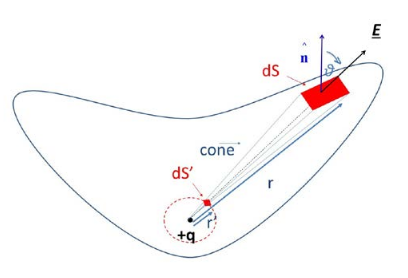
\includegraphics[scale=0.4]{fluxvec.png}
    \end{center}
\end{wrapfigure}
The cone first passes through a sphere centred about the charge and then through the surface of the arbitrary closed shape.

Consider first the sphere: \\
The electric field, $E(r')$, has constant magnitude over the surface of the sphere and is everywhere parallel to $d\unl{S}'$, i.e. $\hn\,dS'$ so we have:
\begin{equation}
    \int \uE(r') \cdot d\unl{S}' = \frac{q}{4\pi\eno(r')^2}\cdot 4\pi(r')^2 = \frac{q}{\eno}
\end{equation}
Consider now the flux through the elemental area $dS$, which is part of the surface of the arbitrary shape surrounding the charge.
We have:
\begin{equation}
    \uE(\unl{r})\cdot \hn\;dS = |E(r)||\hn||\cos\theta|dS
\end{equation}
Since $dS$ is a projection of $dS'$ (because they are both bound by the same cone), we can relate the two of them using:
\begin{equation}
    \frac{dS'}{\pi(r')^2} = \frac{dS}{\pi r^2}\cos\theta
\end{equation}
Substituting, we have:
\begin{align}
    \uE(r)\cdot\hn\;dS &= E(r)\frac{r^2}{(r')^2}dS' \\
    &= \frac{q}{4\pi\eno r^2}\frac{r^2}{(r')^2} dS' \\
    &= \frac{q}{4\pi\eno(r')^2}dS'
\end{align}
Hence the flux through the surface $dS$ is the same as the flux through $dS'$. \\
Integrating gives:
\begin{equation}
    \int \uE\cdot d\unl{S} = \frac{q}{\eno}
\end{equation}
Applying superposition to a collection of charges inside the arbitrary shape gives:
\begin{equation}
    \int \uE\cdot d\unl{S} = \frac{\sum q}{\eno} = \frac{1}{\eno}\int \rho\;dV \tag{Gauss' Law}
\end{equation}
Where $\rho$ is the charge density and then we can use the divergence theorem:
\begin{equation}
    \int \del \cdot \uE dV = \frac{1}{\eno} \int \rho\;dV
\end{equation}
Since the volume integrals are equal for any arbitrary volume, the integrands must also be equal so:
\begin{equation}
    \del \cdot \uE = \frac{\rho}{\eno} \tag{M\RN{1}}
\end{equation}
We conclude that Maxwell's 1st equation is a differential form of Gauss' Law, which in turn is a form of Coulomb's Law. \\
Coulomb's Law (or equivalently Gauss' Law) is only true under static conditions.
Just as with Hooke's Law, experimentation shows us that M\RN{1} is true under all conditions.

The $\uE$-field resulting from any charge distribution gives $\del \cdot \uE = 0$ in the local regions where there is no charge.

\chapter{}
\section{Applying M1 to a Capacitor Plate}
\begin{wrapfigure}{r}{0.4\textwidth}
    \begin{center}
        \vspace{-20pt}
        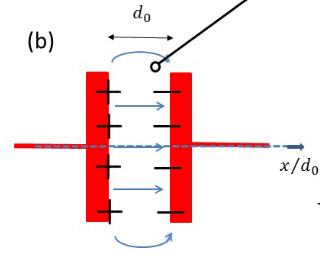
\includegraphics[scale=0.4]{cap.png}
        \vspace{-90pt}
    \end{center}
\end{wrapfigure}
There is no charge density so:
\begin{align}
    \del\cdot\uE &= \frac{\p E_x}{\p x} + \frac{\p E_y}{\p y} + \frac{\p E_z}{\p z} \\
    \del\cdot\uE &= \frac{1}{r^2}\frac{\p}{\p r}(\underbrace{r^2 E_r}_{= 0\text{ (Coulomb)}}) + \frac{1}{r\sin\theta}\frac{\p}{\p \theta}\left[E_\theta\sin\theta\right] + \frac{1}{r\sin\theta}\frac{\p}{\p \phi}(E_\phi) = 0
\end{align}

\subsection{Comments}
\begin{itemize}
    \item $\del\cdot\uE$ describes the spatial dependence of the $\uE$-field
    \item $\del\cdot\uE = 0$ is true at every point where there is no charge
    \item $\del\cdot\uE = 0$ does not necessarily imply $\uE = 0$
    \item $\del\cdot\uE = 0$ can result from any superposition of diverging $\uE$-fields from isolated charges where $\uE$ is exactly proportional to $\frac{1}{r^2}$
    \item Understanding the physics helps to understand the mathematics
\end{itemize}

\section{Maxwell 2 (No magnetic monopole)}
\subsection{Ampere's Law}
Ampere found that two parallel straight wires carrying currents $I_1$ and $I_2$ in the same direction lead to a force $F_2$ on a length L of the wire carrying $I_2$ where
\begin{equation}
    \unl{F}_2 = -\frac{\mu_0 I_1 I_2 L}{2\pi d}\hr_{1\to2} \tag{A}
\end{equation}
and d is the separation between the wires.

We can introduce a magnetic field, where
\begin{equation}
    \unl{F} = q(\unl{v}\times\uB). \tag{B}
\end{equation}
Given that the definition of current is the charge that passes per second,
\begin{equation}
    I = Q_L\cdot v \tag{C}
\end{equation}
where $Q_L$ is the charge per unit length, and v is the velocity of charges. \\
Comparing A and B with C:
\begin{equation}
    \int \uB \cdot d\unl{l} = \mu_0 I \tag{Ampere's Law}
\end{equation}
where I is the current that passes through the surface that is bounded by the path integral of the magnetic field.
\begin{align}
    \int \uB\cdot d\unl{l} &= \uB\cdot2\pi r = \mu_0 I \\
    \implies \uB &= \frac{\mu_0 I}{2\pi r}\hat{\phi} \\
\end{align}

\subsection{Maxwell 2 from the Biot-Savart Law}
Ampere's Law can be written in the form of the Biot-Savart Law that describes the small field ($\delta\uB$) produced by a small length of a current element ($I\,d\unl{l}$) where:
\begin{align}
    \delta \uB = \frac{\mu_0 I}{4\pi r^2}\delta\unl{l} \times \hr &= \frac{\mu_0 I}{4\pi r^2}\sin\theta\,dl\,\hat{\phi} \\
    \del \cdot (\delta\uB) = \frac{1}{\rho}\frac{\p(\rho\,\delta B_\rho)}{\p \rho} &+ \frac{1}{\rho}\underbrace{\frac{\p\, \delta B_\phi}{\p \phi}}_{= 0 \text{ (B-S)}} + \frac{1}{r\sin\theta} \frac{\p}{\p \theta}(\delta B_z) = 0 \\
    \del\cdot(\delta\uB) &= 0 \\
    \sum \delta\uB &= \uB
\end{align}
This leads to Maxwell's second equation:
\begin{equation}
    \del\cdot\uB = 0 \tag{M\RN{2}}
\end{equation}
The net flux through both surfaces is zero. \\
Integrating Maxwell \RN{2}:
\begin{equation}
    \int \del\cdot\uB\,dV = \int 0\cdot dV \implies \int \uB\cdot d\unl{S} = 0
\end{equation}
Hence in all experiments to date, we have found that the net magnetic flux through any closed surface is zero.

\chapter{}
\section{Maxwell 3 from Faraday's Law}
\subsection{Faraday's Fabulous Experiments}
\begin{itemize}
    \item \unl{Inductive Electromotive Force}: \\
    The voltage difference across a single loop wrapped around a coil (or solenoid) is:
    \begin{equation}
        V = \frac{d\uB}{dt}\unl{S} = \frac{\p \phi_{\B}}{\p t}, \tag{Faraday's Law of Induction}
    \end{equation}
    where $\phi_\B$ is the flux of the magnetic field.
    Outside the loop, the $\uB$-field is zero, but the changing magnetic field inside the solenoid generates an $\uE$-field outside and inside the solenoid.
    \item \unl{Motional Electromotive Force}: \\
    A loop of wire moving with velocity, $\unl{u}$, down through the homogeneous field produced between the two magnetic pole pieces.
    Using Faraday's Law of Induction,
    \begin{equation}
        V = \frac{\p \phi_{\B}}{\p t} = \B\frac{\p S(t)}{\p t} = \B\unl{u}\omega,
    \end{equation}
    where $S(t)$ is the instantaneous partial area of the loop with magnetic field, $\uB$, passing through it.
    Alternatively, we can think about the Lorentz force on the free positive charges in the wire in the horizontal (bottom) part of the loop of wire.
    The charges build up at one end of wire and the net force on free positive charges is
    \begin{equation}
        \unl{F} = q(\uE + \unl{v}\times\uB).
    \end{equation}
    In equilibrium,
    \begin{equation}
        \uE = -\unl{v}\times\uB.
    \end{equation}
    Therefore the net voltage produced is
    \begin{equation}
        V = -\omega \E = \B u \omega
    \end{equation}
    Maxwell was the first to point out (leading Einstein to relativity) that the voltage generated in the experiment can be explained using two completely different physical explanations.
\end{itemize}
Faraday's experiments demonstrate that the law of induction is correct no matter why the flux changes; whether the loop moves or the pole pieces move.

\subsection{Using Faraday's Law to find Maxwell 3}
Faraday's Law:
\begin{align}
    \xi_t &= -\frac{\p \phi_\B}{\p t} \\
    \xi_t &= \int \uE \cdot d\unl{l} = -V,
\end{align}
where $\xi_t$ is the electromotive force (the tangential force per unit charge, integrated over length, once around the complete circuit). \\
Using Faraday's Law,
\begin{equation}
    \xi_t = \int \uE\cdot d\unl{l} = -\frac{\p \phi_\B}{\p t} = -\frac{\p}{\p t}\int \uB \cdot d\unl{S}.
\end{equation}
Then using Stoke's Theorem:
\begin{equation}
    \int (\del \times \uE) \cdot d\unl{S} = -\frac{\p}{\p t}\int \uB \cdot d\unl{S}
\end{equation}
Therefore, the integrands can be equated to get:
\begin{equation}
    \del \times \uE = -\frac{\p \uB}{\p t} \tag{M\RN{3}}
\end{equation}

\subsection{Comments}
\begin{enumerate}
    \item The curl of $\uE$ is zero outside the coil, but $\uE$ is not zero.
    \item Maxwell \RN{3} is true at all space and time.
\end{enumerate}

\chapter{}
\section{Maxwell 4 from Ampere's Law}
\subsection{Maxwell's Correction to Ampere's Law}
\begin{wrapfigure}{r}{0.4\textwidth}
    \begin{center}
        \vspace{-40pt}
        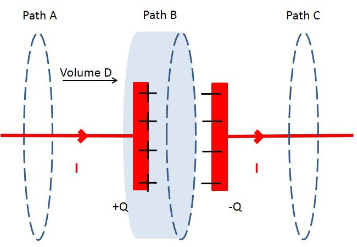
\includegraphics[scale=0.4]{cap4.png}
    \end{center}
\end{wrapfigure}
The surfaces bounded by path $A$ and $C$ each have a current $I$ that threads through them.
Path $B$ has no current threading through it. \\
If Paths $A,B,$ and $C$ are distant from the wire and capacitor, one finds experimentally that the magnetic field is the same at all three. \\
Hence if the moving charges generate both an $\uE$-field and a $\uB$-field (as in the circuit shown), Ampere's Law breaks down. \\
Using Gauss' Law for the $\uE$-field inside the capacitor and consider the volume $D$ that encloses the capacitor plate:
\begin{equation}
    \int \uE \cdot d\unl{S} = \int \frac{\rho}{\eno}dV = \frac{Q}{\eno}
\end{equation}
For the capacitor, using conservation of charge:
\begin{equation}
    I = \frac{dQ}{dt}
\end{equation}
Consider Path $B$:
\begin{align}
    \oint \E \cdot dS &= \int \E \cdot dS \\
    \implies \frac{\p}{\p t} \int \uE \cdot d\unl{S} &= \frac{1}{\eno}\frac{\p Q}{\p t} = \frac{I}{\eno}
\end{align}
Hence, a general equation for Paths $A,B,$ and $C$ is of the form
\begin{equation}
    \int \uB \cdot d\unl{l} = \mu_0 \int \J \cdot d\unl{S} + \mu_0\eno\frac{\p}{\p t} \int \uE \cdot d\unl{S}
\end{equation}
Using Stokes' Theorem:
\begin{equation}
    \int \del \times \uB \cdot d\unl{S} = \mu_0 \int \J \cdot d\unl{S} + \mu_0\eno\frac{\p}{\p t} \int \uE\cdot d\unl{S}
\end{equation}
Given this is true for any surface:
\begin{equation}
    \del \times \uB = \mu_0\J + \mu_0\eno\frac{\p \uE}{\p t} \tag{M\RN{4}}
\end{equation}
where by definition, $\J_{disp} = \eno\frac{\p\uE}{\p t}$, and $\J_{disp}$ is defined as the displacement current density.

From Maxwell's four equations, if we know the charges present and the currents flowing, we can calculate all the $\uE$-fields and $\uB$-fields in a system.

\section{Transverse Electromagnetic Waves and Charge Conservation}
\subsection{Electromagnetic wave in a vacuum}
If we assume that there are no charges or currents present,
\begin{align}
    \del \cdot \uE &= \frac{\rho}{\eno} = 0 \\
    \del \cdot \uB &= 0 \\
    \del \times \uE &= -\frac{\p \uB}{\p t} \\
    \del \times \uB &= \mu_0\eno\frac{\p\uE}{\p t}
\end{align}
Take the curl of Maxwell \RN{3}:
\begin{equation}
    \del \times \del \times \uE = -\frac{\p}{\p t} \del \times \uB
\end{equation}
Use the vector identity:
\begin{align}
    \del \times \del \times \uE &= \del(\del\cdot\uE) - \nabla^2\uE \\
    \nabla^2 &= \frac{\p^2}{\p x^2} + \frac{\p^2}{\p y^2} + \frac{\p^2}{\p z^2} \\
    \implies \nabla^2\uE &= \mu_0 \frac{\p^2 \uE}{\p t^2} \\
    \implies c &= \frac{1}{\sqrt{\mu_0\eno}}
\end{align}
Maxwell used measurements from Weber and Kohlrausch available and found that
\begin{equation}
    c_{Maxwell} = 3.11\times10^8 \,m\,s^{-1}
\end{equation}
The best optical data (Foucault) gave
\begin{equation}
    c_{Foucault} = 2.98\times10^8\,m\,s^{-1}
\end{equation}

\chapter{}
Using the curl of Maxwell \RN{4}:
\begin{equation}
    \nabla^2\uB = \mu_0\eno\frac{\p^2\uB}{\p t^2}
\end{equation}

\section{The Vectorial Nature of Electromagnetic Waves}
Given that $\uE$ and $\uB$ are plane waves of the form:
\begin{align}
    \uE(\vec{r},t) &= \uE_0\exp(i[\vk\cdot\vec{r}-\omega t]) \\
    \uB(\vec{r},t) &= \uB_0\exp(i[\vk\cdot\vec{r}-\omega t])
\end{align}
$\uE_0$ and $\uB_0$ are the polarisation vectors for $\uE$ and $\uB$, and $\vk$ gives the magnitude of the wave-vector and direction of propagation. \\
There are non-trivial (i.e. real) solutions only if $\omega$ and $\vk$ are the same for $\uE$ and $\uB$.
The solution for the wave equation for electromagnetic waves can be written as:
\begin{align}
    \vk\cdot\vk &= k^2 = \omega^2\mu_0\eno \\
    \implies v_{phase} &= f\lam = \frac{\omega}{k} = \sqrt{\frac{1}{\mu_0\eno}}
\end{align}
Substituting the plane wave solutions into Maxwell \RN{3}:
\begin{align}
    \del \times \uE = i\vk \times \uE &= -\frac{\p\uB}{\p t} = i\omega\uB \\
    \implies i\vk\times\uE_0 &= i\omega\uB_0
\end{align}
Similarly from Maxwell \RN{4}:
\begin{equation}
    \vk \times \uB_0 = -\mu_0\eno\omega\uE_0
\end{equation}

\subsection{Implication}
\begin{itemize}
    \item $\uE, \uB,$ and $\vk$ are all orthogonal to each other in a vacuum
    \item $|\uB_0|$ is a factor of $c$ smaller than $|\uE_0|$
    \item $\uE_0\times\uB_0$ is in the direction of $\vk$ which is the direction of propagation
\end{itemize}

\section{Dispersive and Ballistic Motion of Waves}
\begin{itemize}
    \item Ballistic motion does not change as it moves through space (ball flying through air)
    \item Dispersive motion changes as it moves through space (ripple on pond)
\end{itemize}
\begin{enumerate}
    \item The phase velocity (of each component of a disturbance) is:
    \begin{equation}
        v_{phase} = f\lam = \frac{\omega}{k},~ k \in \mathbb{R}
    \end{equation}
    \item The group velocity for a disturbance is determined by how the peak of the disturbance moves through space as a function of time.
    \begin{equation}
        v_{group} = \frac{\p\omega}{\p k}\Bigg|_{k = k_0}, ~ k_0 = \text{average value}
    \end{equation}
    \item If the motion is ballistic:
    \begin{equation}
        \frac{\p^2\omega}{\p k^2} = 0
    \end{equation}
    If the motion is dispersive:
    \begin{equation}
        \frac{\p^2 \omega}{\p k^2} \neq 0
    \end{equation}
\end{enumerate}

\section{Electromagnetic Waves in Insulators and Conductors}
We can use Maxwell's equations and Ohm's Law to describe electromagnetic waves propagating through metals. \\
Taking the curl of Maxwell \RN{3}:
\begin{equation}
    \del \times \del \times \uE = -\frac{\p}{\p t}\del \times \uB
\end{equation}
Substituting Ohm's Law ($\J = \sigma_N\uE$) into Maxwell \RN{4} gives:
\begin{align}
    \del\times\uB &= \mu_0\J + \mu_0\eno\frac{\p \uE}{\p t} \\
    &= \mu_0\sigma_N\uE + \mu_0\eno\frac{\p\uE}{\p t} \\
    \del \times \del \times \uE &= -\mu_0\sigma_N\frac{\p\uE}{\p t} - \mu_0\eno\frac{\p^2\uE}{\p t^2}
\end{align}
Using the vector identity:
\begin{align}
    \del\times\del\times\uE &= \cancel{\del(\del\cdot\uE)} - \nabla^2\uE \\
    \implies \nabla^2\uE &= \mu_0\sigma_N\frac{\p\uE}{\p t} + \mu_0\eno\frac{\p^2\uE}{\p t}
\end{align}
We assume:
\begin{equation}
    \uE(\vec{r},t) = \uE_0\exp(i[\vk\cdot\vec{r}-\omega t])
\end{equation}
Note: $\omega$ is always real and constant. \\
We allow $\vk$ to be a complex vector.
When $\vk$ has both real and imaginary parts, the wave is both oscillating and decaying. \\
Substituting into the wave equation:
\begin{equation}
    k^2 = \mu_0\eno\omega^2 + i\omega\mu_0\sigma_N \tag{Dispersion Relation}
\end{equation}
A dispersion relation is one that gives us $\omega$ vs $\vk$.

\begin{enumerate}
    \item For a highly insulating material,
    \begin{align}
        \sigma_N &\to 0 \\
        \implies k^2 &= \mu_0\eno\omega^2 \\
        \implies k &= \sqrt{\mu_0\eno}\omega \\
        \implies v_{phase} &= \frac{\omega}{k} = \frac{1}{\sqrt{\mu_0\eno}}
    \end{align}
    \item For a highly conducting material,
    \begin{align}
        \sigma_N &\to \infty \\
        \implies k^2 &= i\omega\mu_0\sigma_N \\
        \sqrt{i} &= \frac{1 + i}{\sqrt{2}} \\
        \implies k &= (1 + i)\sqrt{\frac{\omega\mu_0\sigma_N}{2}} = \frac{1 + i}{\delta}, ~\delta = \sqrt{\frac{2}{\omega\mu_0\sigma_N}}
    \end{align}
    The solution is found by simply substituting back into the plane wave equation:
    \begin{align}
        \uE &= \uE_0\exp\left[i\left(\left(\frac{1 + i}{\delta}\right)x - \omega t\right)\right] \\
        &= \uE_0\exp\left[i\left(\frac{x}{\delta} - \omega t\right)\right]\exp\left(-\frac{x}{\delta}\right)
    \end{align}
\end{enumerate}

\chapter{}
\begin{align}
    k &= (1 + i)\sqrt{\frac{\om\mu_0\sigma_N}{2}} = \frac{1 + i}{\delta} \\
    \uE &= \uE_0 \exp\left[i(kx - \om t)\right] \\
    &= \uE_0\exp\left[i\left(\frac{1+i}{\delta}x - \om t\right)\right] \\
    &= \uE_0\exp\left[i\left(\frac{x}{\delta} - \om t\right)\right]\exp\left(-\frac{x}{\delta}\right)
\end{align}
We extract the important physics by taking the real of imaginary part of $\uE$.\\
The real part:
\begin{equation}
    \uE = \uE_0\cos\left(\frac{x}{\delta}- \om t\right)\exp\left(-\frac{x}{\delta}\right)
\end{equation}
The wavelength, $\lam = \frac{2\pi}{k_{real}} = 2\pi\delta$, and the decay length (known as the 'skin depth' for highly conducting materials), $\delta = \frac{1}{k_{\mathbb{C}}}$

For copper at optical frequencies:
\begin{equation}
    \delta = \sqrt{\frac{2}{\om\mu_0\sigma_N}} = 4\,nm
\end{equation}

\section{The continuity equation and charge conservation}
Maxwell \RN{4}:
\begin{align}
    \del\times\uB &= \mu_0\J + \mu_0\eno\frac{\p\uE}{\p t} \\
    \del\cdot\del\times\uB &= \mu_0\del\cdot\J + \mu_0\eno\frac{\p}{\p t}\del\cdot\uE \\
    \implies \del\cdot\J &= -\mu_0\eno\frac{\p}{\p t}\underbrace{\del\cdot\uE}_{M\RN{1}}
\end{align}
\begin{equation}
    \del\cdot\J = -\frac{\p\rho}{\p t} \tag{Continuity Equation}
\end{equation}
Take the volume integral of both sides:
\begin{align}
    \int \del\cdot\J\;dV &= -\int \frac{\p\rho}{\p t}\,dV \\
    \int \J \cdot d\unl{S} &= -\int \frac{\p\rho}{\p t}\,dV \\
    \text{Charge flowing out through the surface every second } &= \text{ Change in total charge inside the volume every second}
\end{align}
Hence the continuity equation is equivalent to conservation of charge $\implies$ Maxwell's equations require the conservation of charge.

\section{Maxwell and Einstein}
\subsection{The Collapse of Newtonian/Galilean Physics}
\begin{enumerate}
    \item observer P: stationary with respect to positive charges, sits on positive charges and watches negative charges move past with velocity, $v$
    \begin{equation}
        \unl{F} = q(\uE + \unl{v}\times\uB)
    \end{equation}
    For a charge-neutral wire and an external charge that is not moving, $\unl{F} = 0$, this implies the test charge does not move.
    \item observer N: stationary with respect to the negative charges, observes positive charges move past with velocity, $v$
    \begin{equation}
        \unl{F} = q(\uE + \unl{v}\times\uB)
    \end{equation}
    For a charge-neutral wire, we again assume the electric field is zero.
    However, $\unl{v}$ and $\uB$ are non-zero, so N concludes that Maxwell's equations predict the positive test charge moves towards the wire.
\end{enumerate}
If we assume the wire is charge-neutral in both frames, Maxwell's equations give a contradiction. \\
Assume that for observer N, the wire is charge-neutral (i.e. in the rest frame of the battery).
\begin{align}
    I &= n_1ev \\
    \uB &= \frac{\mu_0I}{2\pi r}\hat{\phi} = \frac{\mu_0 n_1ev}{2\pi r}\hat{\phi} \\
    F &= q\unl{v}\times\uB \\
    \implies \unl{F}_N &= -\frac{\mu_0 qn_1ev^2}{2\pi r}\hr
\end{align}

\chapter{}
For Observer P, there is a Lorentz contraction of the moving negative charges:
\begin{equation}
    \lam_{-ve} = -\gamma n_2e
\end{equation}
where $\lam$ is the charge per unit length, $\gamma = \frac{1}{\sqrt{1 - \tfrac{v^2}{c^2}}}$. \\
Observer P also says that given there is charge neutrality for Observer N,
\begin{align}
    \lam_{+ve} &= \frac{n_1 e}{\gamma} \\
    \implies \lam_{total} &= -\gamma n_2e \left(1 - \frac{1}{\gamma^2}\right) = -\gamma n_2e\frac{v^2}{c^2}
\end{align}
From Gauss' Law:
\begin{align}
    \implies \uE_p &= \frac{\lam_{total}\hr}{2\pi\eno r} \implies \uE_p = -\frac{\gamma \mu_0n_2ev^2}{2\pi r}\hr \\
    \implies F_p &= q\uE_p = \gamma q\unl{v} \times \uB = \gamma \unl{F}_n
\end{align}
The force that was purely magnetic for observer N is purely electrostatic for observer P.
They both agree the positive charge crashes into the wire.

Observer N is in the non-accelerating rest frame:
\begin{align}
    \delta t_N &= \gamma \delta t_P \\
    F_p &= \frac{\p P_p}{\p t_p} ~;~ F_N = \frac{\p P_N}{\p t_N} \\
    \implies \delta P_p &= \delta P_N
\end{align}
The two observers agrees that the change in momentum is the same in the direction orthogonal to the motion, as required by relativity.

There are parallels between the roles of the charges and the battery with Einstein's twin paradox.
Observer N is in the rest frame of the battery.
This is analogous to the twin that stays at home.

Coulomb's law can be regarded as fundamental with magnetic forces and induced EMF being relativistic corrections to this.

\section{Bulk Properties of Conductors, Dielectrics, and Magnetic Materials}
\subsection{Electrical Conductors}
\textbf{Microscopic properties for conductors}
\begin{itemize}
    \item Drude Model is that the electric field accelerates the charges which then collide with the scattering sites.
    \item Take $N$ to be the number of charges per unit volume; $q$ to be the charge on each carrier; and $\tau$ as the scattering time:
    \begin{equation}
        \rho_N = \frac{m}{Nq^2\tau}
    \end{equation}
\end{itemize}

\textbf{Extensive and Intensive Variables}
\begin{equation}
    V = IR \tag{Ohm's Law}
\end{equation}
\begin{itemize}
    \item[R] - extensive property which depends on the amount and the shape of the material being measured.
\end{itemize}
Rewriting Ohm's Law:
\begin{align}
    \frac{V}{L} &= \frac{I}{A} \cdot \frac{RA}{L} \\
    E &= J \rho_N
\end{align}
This defines resistivity as an intensive variable \\
By definition, $\rho_N = \frac{1}{\sigma_N}$, where $\sigma_N$ is the conductivity.

\textbf{Current Densities and Charge Densities}
\begin{equation}
    \J = \sigma_N \uE \tag{Current Density}
\end{equation}
In general, the movement of bulk charge density in conductors is so fast that we can assume to a good approximation that $\rho = 0.$

Using Ohm's Law, Maxwell \RN{1}, and the continuity equation, we can use a dimensionality argument to find
\begin{equation}
    \tau = \rho_N\eno
\end{equation}
For copper, $\rho_N \approx 10^{-8}\,\Omega m$, we find that $\tau$ (characteristic time for charge density to change) is $\approx 10^{-20}\,s$.
This can be compared to the inverse frequency for light - $3\times10^{-15}\,s$

\chapter{}
\section{Dielectrics}
\subsection{Microscopic Properties and Definitions for Dielectrics}
\begin{enumerate}
    \item \unl{Polar Dielectrics}: e.g. water
    \begin{itemize}
        \item A permanent dipole moment.
        \item Increasing the $\uE$-field increases the number of dipoles that overcome the randomising effects of temperature so they rotate into the direction of the applied field.
    \end{itemize}
    \item \unl{Non-Polar Dielectrics}: e.g. Ar, CO$_2$
    \begin{itemize}
        \item Increasing the $\uE$-field causes separation of positive and negative charges.
    \end{itemize}
\end{enumerate}
Dielectrics produce their own electric field, with the fundamental response of a dielectric:
\begin{equation}
    p = q\unl{d}
\end{equation}
This is the definition of the elementary dipole moment, $\unl{p}$
\begin{equation}
    \unl{P} = N\unl{p}
\end{equation}
This is the definition of polarisation ($C\,m^{-2}$), where $N$ is the number of dipole moments per unit volume.

How we characterise bulk dielectric materials is a matter of taste:
\begin{enumerate}
    \item Definition of relative dielectric constant, $\er$ (dimensionless)
    \begin{equation}
        \unl{P} = \eno(\er - 1)\uE
    \end{equation}
    \item Definition of electric susceptibility, $\chi_e$ (dimensionless)
    \begin{equation}
        \unl{P} = \eno\chi_e\uE
    \end{equation}
\end{enumerate}
$\unl{D}$ is a useful shorthand used in many calculations (no new Physics)
\begin{equation}
    \unl{D} = \eno\uE + \unl{P}
\end{equation}
This is the definition of $\unl{D}$, the electric displacement field

\subsection{Current Density and Charge Density in Dielectrics}
In an applied $\uE$-field, we can consider negative charges as displaced.
The positive in the sheet at $(x+\delta x, y, z)$ is:
\begin{equation}
    Q_{+ve} = \underbrace{Nq}_{C/V} \cdot \underbrace{Sd}_{V \text{ of }+ve}
\end{equation}
which can be written in terms of surface charge density, $\sigma$:
\begin{equation}
    \sigma = \frac{Q_{+ve}}{S} = Nqd = \unl{P}
\end{equation}
More generally, the surface charge density is:
\begin{equation}
    \sigma = \unl{P}\cdot\hn
\end{equation}

Consider a cube of non-uniform polarisation:

\begin{wrapfigure}{r}{0.42\textwidth}
	\centering
	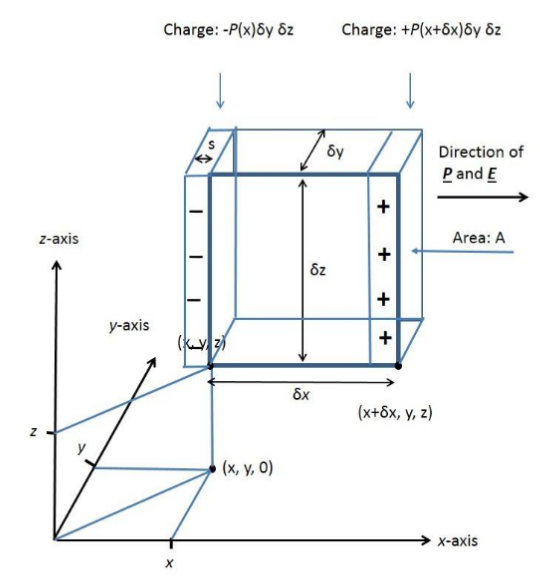
\includegraphics[scale=0.38]{dibox.png}
\end{wrapfigure}

The negative charge that leaves the cube across the interface at $x$ is given by:
\begin{equation}
    Q_{out} = -P(x)\,\Delta y \,\Delta z
\end{equation}
The negative charge that moves into the cube from the neighbouring cube is:
\begin{equation}
    Q_{in}(x+\delta x) = -P(x+\delta x)\,\Delta y \, \Delta z
\end{equation}
The net increase in (positive) charge in the cube is:
\begin{equation}
    Q_{net} = -\left[P(x_\delta x)-P(x)\right]\,\Delta y\,\Delta z = -\frac{\p P}{\p x} \delta x \, \delta y \, \delta z
\end{equation}
Using similar logic for the y and z directions, the (bound) charge density is:
\begin{equation}
    \rho = -\frac{\p P_x}{\p x} - \frac{\p P_y}{\p y} - \frac{\p P_z}{\p z} = -\del\cdot\unl{P}
\end{equation}

\chapter{}
\begin{equation}
    \underbrace{\rho_b}_{\text{bound}} = -\del\cdot\unl{P}
\end{equation}
Consider an arbitrary volume of polarised material.
If the polarisation changes as a function of time, the moving charges are equivalent to the current.
The charge flowing out of the arbitrary volume is
\begin{align}
    \frac{\p Q_{out}}{\p t} &= -\int \frac{\p \rho_{in}}{\p t}dV \\
    &= \frac{\p}{\p t} \int \del\cdot\unl{P}\,dV = \frac{\p}{\p t}\int \unl{P}\cdot d\unl{S} \\
    &= \frac{\p}{\p t} \int \unl{P} \cdot d\unl{S} - \int \J_b \cdot d\unl{S}, ~ \J_b - \frac{\p \unl{P}}{\p t}
\end{align}
Summary: \\
For a dielectric, once we have $\unl{P}$, we have
\begin{align}
    \sigma &= \unl{P}\hn = \eno(\er - 1)\uE\cdot \hn \\
    \rho_b &= -\del\cdot\unl{P} = -\eno(\er - 1)\del\cdot\uE \\
    \J_b &= \frac{\p \unl{P}}{\p t} = \eno(\er - 1)\frac{\p\uE}{\p t}
\end{align}
How are these results useful? M\RN{3} \& \RN{4}:
\begin{align}
    \del\times\uE &= -\frac{\p\uB}{\p t} \\
    \del\times(\del\times\uE) &= -\frac{\p}{\p t}\del\times\uB \\
    \del\times\uB &= \mu_0\J + \mu_0\eno\frac{\p \uE}{\p t} \\
    &=\mu_0\left(\sigma_N\uE + \eno(\er - 1)\frac{\p\uE}{\p t}\right) + \mu_0\eno\frac{\p \uE}{\p t}
\end{align}
Substituting and using the vector identity for $\del\times\del\times\uE \implies$
\begin{equation}
    \del^2\uE = \mu_o\sigma_N \frac{\p\uE}{\p t} + \mu_0\eno\er\frac{\p^2\uE}{\p t^2}
\end{equation}
This is the wave equation for a conducting dielectric.

\section{Magnetic Materials}
\subsection{Microscopic Properties and Definitions}

A magnetic material produces its own magnetic field.

Consider Ampere's model for a magnetic material:
\begin{itemize}
    \item Each atom has electrons orbiting that produce a small magnetic field
    \item Applying a magnetic field tends to align the magnetic moments with the applied $\uB$-field
\end{itemize}
A quantum mechanical picture gives some similar ideas where we consider the occupation of quantum states with different magnetic properties.
\begin{equation}
    \unl{m} = IS\hn
\end{equation}
\textbf{Note:} \textit{$\unl{m}$ is the magnetic moment, be careful of getting confused with other $m$s in Physics.}

The fundamental response of magnetic material:
\begin{equation}
    \unl{m} = IS\hn
\end{equation}
This is the definition of the magnetic dipole moment, where a current $I$ flows around a loop of area $S$.
\begin{equation}
    \unl{M} = N\unl{m}
\end{equation}
This is the definition of magnetisation ($\unl{M}$), where $N$ is the number of dipoles per unit volume.

\textbf{Note:} \textit{$\unl{H}$ is a useful shorthand commonly used in calculations (no new Physics).}
\begin{equation}
    \uB = \mu_0(\unl{H} + \unl{M})
\end{equation}
This is the definition of $\unl{H}$, the magnetic field strength.

How we characterise bulk magnetic materials is a matter of taste:
\begin{enumerate}
    \item Definition of susceptibility, $\chi$:
    \begin{equation}
        \unl{M} = \chi \unl{H}
    \end{equation}
    \item Definition of permeability, $\mu_r$:
    \begin{equation}
        \uB = \mu_0\mu_r\unl{H}
    \end{equation}
\end{enumerate}
For a magnetised cylinder,
\begin{align}
    \uB &= \uB_{\text{applied}} + \underbrace{\mu_0\unl{M}}_{\text{material field}} \\
    \implies \mu_0\unl{H} &= \uB_{\text{applied}}
\end{align}

\begin{figure}[H]
	\centering
	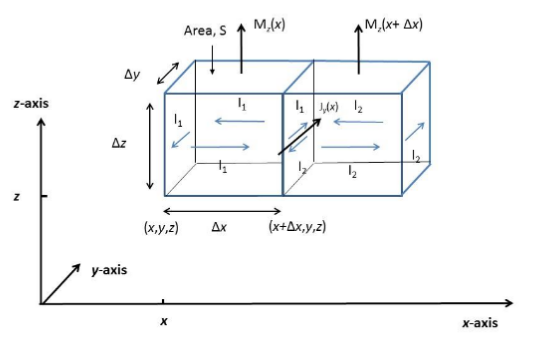
\includegraphics[scale=0.4]{magbox1.png}
	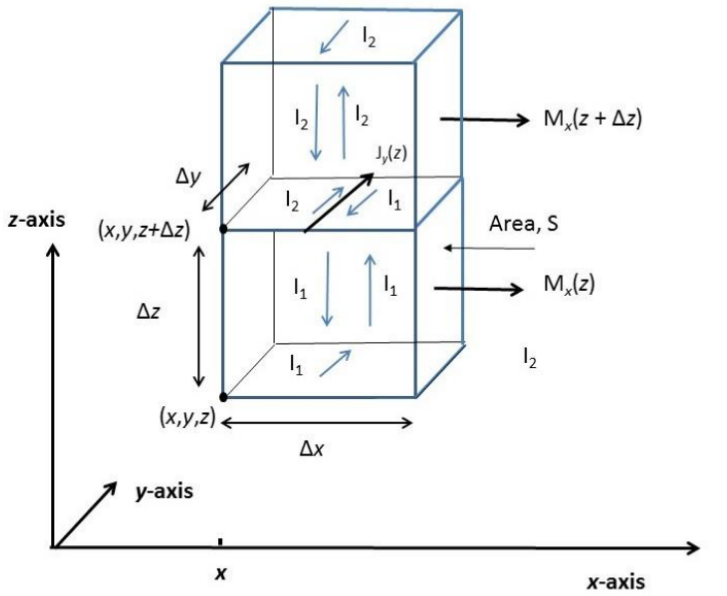
\includegraphics[scale=0.3]{magbox2.png}
\end{figure}

Consider the currents flowing:
\begin{align}
    m_z(x) &= M_z(x)\,\Delta x\,\Delta y\,\Delta z \\
    &= I_1(x)S = I_1(x)\,\Delta x\,\Delta y \\
    \implies I_1(x) &= M_z(x)\,\Delta z
\end{align}

\chapter{}
\begin{align}
    m_z(x) &= M_z(x)\,\Delta x\,\Delta y\,\Delta z \\
    &= I_1(x)S = I_1(x)\,\Delta x\,\Delta y \\
    \implies I_1(x) &= M_z(x)\,\Delta z
\end{align}
The current flowing along the interface between the cubes ($I_{net}$):
\begin{align}
    I_{net} &= M_z\,\Delta z - [M_z(x + \Delta x)\,\Delta z] = -\Delta M_z\,\Delta z \\
    &= -\frac{\Delta M_z}{\Delta x} \Delta x\, \Delta z \\
    \implies J_y &= \frac{I_{net}}{\Delta x\,\Delta z} = - \frac{\Delta M_z}{\Delta x} \\
    \implies J_y &= -\frac{\p M_z}{\p x}
\end{align}
There is also a contribution to $J_y$ if $M_x$ varies given by:
\begin{equation}
    J_y = \frac{\p M_x}{\p z}
\end{equation}
Hence, in general,
\begin{equation}
    \J = \del \times \unl{M}
\end{equation}

For a uniformly magnetised material, there is a discontinuous change in $\unl{M}$ at the surface.
The current through the rectangle can equally well be considered as a surface current per unit length or a bulk current density ($\J$) where:
\begin{align}
    \int \J\cdot d\unl{S} &= I_LL \\
    \J &= \del \times \unl{M} \\
    \int \J\cdot d\unl{S} &= \int (\del\times\unl{M})\cdot d\unl{S} = \int \unl{M}\cdot d\unl{l} \\
    &= ML = I_LL \\
    \implies M &= I_L \\
    \implies \unl{I}_L &= \unl{M}\times\hn
\end{align}
Hence, if we know $\unl{M}$, we know the surface current per unit length, $\M \times \hn$, and the bulk current density, $\del\times\M$

\section{Propagation of Transverse EM Waves in Materials}
\subsection{General Dispersion Relation for an Infinite Linear Isotropic Homogeneous Medium}
We can derive the general dispersion relation using Maxwell \RN{4}:
\begin{align}
    \del\times\uB &= \mu_0\J + \mu_0\eno\frac{\p\uE}{\p t}
\end{align}
The total current density (for ILIH):
\begin{align}
    \J_{\text{total}} &= \J_{\text{free}} + \J_{\text{bound}} \\
    \J_{\text{free}} &= \J_{\text{Ohm}} + \J_{\text{experiment}} \\
    \J_{\text{bound}} &= \frac{\p \unl{P}}{\p t} + \del\times\M
\end{align}
Charge density ($C\,m^{-3}$): Insulating dielectrics give a surface charge density ($\unl{P}\cdot\hn$) and a volume charge density ($-\del\cdot\unl{P}$).\\
For a wave travelling through an ILIH medium, in general we can write:
\begin{align}
    \del\cdot\uE &= \frac{\rho_{\text{free}}+\rho_{\text{bound}}}{\eno} = \frac{\rho_{\text{free}}}{\eno} - (\er - 1)\del\cdot\uE \\
    \implies \del\cdot\uE &= \frac{\rho_{\text{free}}}{\er\eno} = 0
\end{align}
This condition holds as long as the frequency of the wave is sufficiently low that the charge density associated with the conducting medium is zero.

Maxwell \RN{4} can be written as
\begin{equation}
    \del\times\uB = \mu_0\underbrace{\left(\sigma_N \uE + \frac{\p \unl{P}}{\p t} + \del\times\M\right)}_{\J_{\text{total}}} + \mu_0\eno\frac{\p \uE}{\p t}
\end{equation}
This can be rearranged:
\begin{align}
    \del\times(\uB - \mu_0\M) = \mu_0\sigma_N\uE + \mu_0\frac{\p}{\p t}(\unl{P} + \eno\uE)
\end{align}
Using the materials' definitions:
\begin{align}
    \unl{P} &= \eno(\er - 1)\uE \\
    \uB &= \mu_0(\unl{H}+\M) = \mu_0\mu_r\unl{H}
\end{align}
Maxwell \RN{4} can be rewritten as
\begin{equation}
    \del\times\frac{\uB}{\mu_r} = \mu_0\sigma_N\uE + \mu_0\frac{\p}{\p t} (\eno\er\uE)
\end{equation}
Now substitute this into the curl of Maxwell \RN{3} to find:
\begin{align}
    \del\times(\del\times\uE) = -\frac{\p}{\p t}(\del\times\uB) = -\frac{\p}{\p t}\left[\mu_0\mu_r\left(\sigma_N\uE + \eno\er\frac{\p \uE}{\p t}\right)\right]
\end{align}
Using $\del\times\del\times\uE = \del(\del\cdot\uE) - \del^2\uE$:
\begin{align}
    \del^2\uE - \mu_0\mu_r\sigma_N\frac{\p \uE}{\p t} - \mu_0\mu_r\eno\er\frac{\p^2\uE}{\p t^2} = 0
\end{align}

\chapter{}

\begin{itemize}
    \item $\mu_0\mu_r \to \mu$
    \item $\eno\er to \e$
\end{itemize}
\begin{equation}
    \del^2\uE - \mu\sigma_N\frac{\p \uE}{\p t} - \mu\e\frac{\p^2\uE}{\p t^2} = 0
\end{equation}
Equally taking the curl of M\RN{4} gives:
\begin{equation}
    \del^2\uB - \mu\sigma_N \frac{\p \uB}{\p t} - \mu\e\frac{\p^2\uB}{\p t^2} = 0
\end{equation}
We can substitute a plane wave solution into the wave equation:
\begin{align}
    \uE &= \E_0 \exp(i[kx - wt]) \\
    \implies -k^2 &= iw\mu\sigma_N + \mu\e w^2 = 0 \\
    \implies k^2 &= \mu\e w^2 + iw\mu\sigma_N
\end{align}
This is the general dispersion relation for an infinite, linear, isotropic, homogeneous medium.

\begin{example}[Electromagnetic Waves in Conducting/Dielectric/Magnetic Materials]
Use the general dispersion relation to calculate the approximate decay length, wave-vector, and wavelength of a wave of frequency $10^{15}Hz$ propagating through Tungsten ($\rho_N = 1\,m\Omega\,cm$).
Tungsten is neither magnetic nor a dielectric. \\
Given $f = 10^{15}Hz,\;\rho_N \approx 10^{-5}\Omega\,m,\;\sigma_N = 10^5\,\Omega^{-1}m^{-1},\;\mu=\mu_0,\;\e=\eno$:
\begin{align}
    k^2 &= 4\pi\times10^{-7}\cdot8.85\times10^{-12}\cdot(2\pi\times10^{15})^2 + i(2\pi\times10^{15})\cdot4\pi\times10^{-7}\times10^5 \\
    &= 4.4\times10^{14} + i7.9\times10^{14}
\end{align}
Note: Tungsten cannot be considered either as a good insulator or as a good conductor \\
Use an argand diagram and find the magnitude of k:
\begin{align}
    \tan\phi &= \frac{7.9}{4.4} \implies \phi = 60.8^\circ \implies \frac{\phi}{2} = 30.4^\circ \\
    |k| &= \Big|(4.4\times10^14)^2 + (7.9\times10^{14})^2\Big|^{1/4} = 3.0\times10^7 \\
    k &= |k|\cos\frac{\phi}{2} + i|k|\sin\frac{\phi}{2} \\
    &= 2.59\times10^7 + i\,1.52\times10^7 \\
    \uE &= \E_0 \exp(i[(2.59\times10^7 + i\,1.52\times10^7)x - wt]) \\
    &= \E_0 \exp(i[2.59\times10^7x - wt])\exp(-1.52\times10^7x)
\end{align}
Taking either the real or imaginary parts gives:
\begin{equation}
    \uE = \E_0 \cos(2.59\times10^7 - wt)\exp(-1.52\times10^7x)
\end{equation}
The wave-vector is the real part of $k$, $2.59\times10^7m^{-1}$ and wavelength, $\lam = \frac{2\pi}{k_{real}} = 2.4\times10^{-7}m$ \\
The decay length is the distance for $\uE$ to decrease by $\frac{1}{e} \implies \delta = \frac{1}{k_{imag}} = 66\,nm$
\end{example}

\section{Advanced Microscopic Descriptions of Conductors, Superconductors, and Dielectrics}
\subsection{Conducting Materials - Metal and Plasma}
We use a stable one-dimensional, scalar, Drude model to describe the scattering of charge carriers.
In the Drude model, the charge carriers accelerate for an average time, $\tau$.
They then scatter and instantaneously stop.
The fraction of charge carriers that scatter in a time $\delta t$ is $\frac{\delta t}{\tau}$, and the remaining fraction that don't scatter is $\left(1 - \frac{\delta t}{\tau}\right)$.
Hence, the momentum of the charge carriers at time $t+\delta t$ is given by:
\begin{equation}
    p(t+\delta t) = \left(1 - \frac{\delta t}{\tau}\right)p(t) + \left(1 - \frac{\delta t}{\tau}\right)f(t)\,\delta t + f(t)\delta t \frac{\delta t}{\tau}
\end{equation}
Three terms:
\begin{enumerate}
    \item Initial momentum at time $t$ of the charge are not scattered
    \item Increase in momentum during the time interval of $\delta t$ of the unscattered carriers
    \item An upper bound for the momentum of the carriers scattered at some point in time during $\delta t$
\end{enumerate}
\begin{align}
    \delta p &= p(t+\delta t) - p(t) \\
    \frac{\delta p}{\delta t} = -\frac{p(t)}{\tau} + f(t) + \cancel{O(\delta t)}
\end{align}
The general expression for the force on a charge carrier:
\begin{equation}
    \unl{F} = m\frac{dp}{dt} = q(\uE + \unl{v}\times\uB)
\end{equation}
In an electromagnetic wave, $\uB \approx \frac{|\E|}{c}$, so $\unl{v}\times\uB \ll \uE$ unless the charge carriers are moving close to the speed of light.
Hence, we neglect the $\unl{v}\times\uB$ term in the expression for the Lorentz force.
Using $F = qE$ and $p = mv$:
\begin{equation}
    m\frac{dv}{dt} = qE - \frac{mv}{\tau} \tag{Equation of Motion}
\end{equation}
where $\frac{mv}{\tau}$ can be considered as a frictional damping term \\
Using $\J = Nq\unl{v}$, where $N$ is the number of charges per unit volume, $q$ is the charge on each carrier, and $\unl{v}$ is the velocity of the carriers, can rewrite as

\chapter{}
\begin{equation}
    m\frac{dJ}{dt} = Nq^2E - \frac{m}{\tau}J
\end{equation}
We assume complex oscillating solutions of the form:
\begin{equation}
    \uE = \uE_0\exp(-i\omega t),~ \J = \J_0\exp(-i(\omega t - \delta))
\end{equation}
where $\delta$ is the phase shift between $\uE$ and $\J$. The differential equation of motion gives
\begin{equation}
    \J = \frac{Nq^2}{m(\tau^{-1} - i\omega)}\uE
\end{equation}
Comparing this expression to the definition for conductivity: $\J = \sigma_N\uE$, gives a complex conductivity:
\begin{equation}
    \sigma_N = \frac{Nq^2}{m(\tau^{-1} - i\omega)}
\end{equation}
\begin{itemize}
    \item Metals (short scattering time): \\
    In the short scattering time limit ($\tau \ll \omega^{-1}$), we find the Drude expression:
    \begin{equation}
        \sigma_N = \frac{Nq^2\tau}{m}
    \end{equation}
    \item Plasma (long scattering time- low density plasma) \\
        A low density plasma is a net neutral system of charged particle (ions and electrons) in which the density of the charged carriers is sufficiently small that the charged carriers don't often collide \\
        Examples:
        \begin{itemize}
            \item Ionised gas in fluorescent lights;
            \item the ionosphere which is a region 100 km to 600 km above the Earth's surface, which is ionised by the radiation from the sun;
            \item the plasma in a fusion energy tokamak;
            \item and some other interstellar media
        \end{itemize}
        Usually, we ignore the response of ions because they are much slower than the electrons to react. In the long scattering time limit:
        \begin{equation}
            \sigma_N = \frac{-Nq^2}{m_ei\omega} = +\frac{iNq^2}{m_e\omega}
        \end{equation}
        Using the dispersion relation
        \begin{equation}
            k^2 = \mu\e\omega^2 + i\omega\mu\sigma_N
        \end{equation}
        Since the plasma is not contained in a magnetic or dielectric medium so $\er = 1$ and $\mu_r = 1$. Hence,
        \begin{align}
            k^2 &= \mu_0\eno\omega^2 + i\omega\mu_0\frac{iNe^2}{m_e\omega} = \mu_0\eno\omega^2 - \frac{\mu_0Ne^2}{m_e} \\
                &= \frac{\omega^2}{c^2}\left(1 - \left(\frac{\omega_p}{\omega}\right)^2\right),~ \omega_p = \sqrt{\frac{Ne^2}{m_e\eno}}
        \end{align}
        The dispersion relation has two regimes:
        \begin{enumerate}
            \item $\omega > \omega_p$: $k$ is real and the electromagnetic waves propagate without attenuation through the plasma
                \begin{equation}
                    v_{phase} = \frac{c}{\sqrt{1 - \left(\frac{\omega_p}{\omega}\right)^2}} > c
                \end{equation}
            \item $\omega < \omega_p$: $k$ is imaginary and there is an attenuated propagation of the electromagnetic wave
                \begin{equation}
                    v_{group} = c\sqrt{1 - \left(\frac{\omega_p}{\omega}\right)^2} < c
                \end{equation}
        \end{enumerate}
\end{itemize}
\begin{figure}[H]
	\centering
	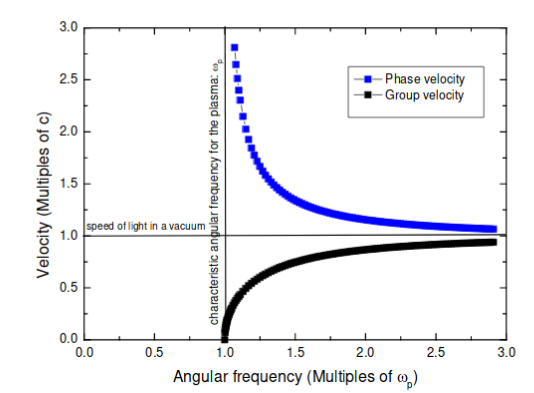
\includegraphics[scale=0.4]{phasegroup.png}
	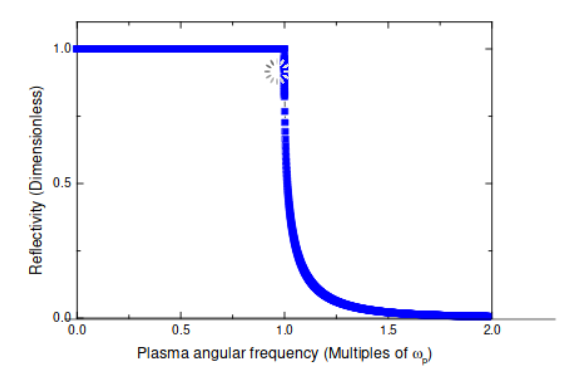
\includegraphics[scale=0.4]{plasma.png}
\end{figure}

\section{Superconducting Materials}
Applications:
\begin{itemize}
    \item MRI body scanners;
    \item Particle accelerators;
    \item fusion energy tokamaks;
    \item voltage standards;
    \item in the future, power transmission
\end{itemize}
There is no simple model for zero resistivity in superconductivity.
We can think about superconductors as the condensation of the normal electrons of a metal into a ground state.
The ground state has an associated energy.
The superelectrons are not scattered (i.e. zero resistivity).
We can think of a superconductor as being like an enormous atom with a (macroscopic) wavefunction that can be kilometres long.

\chapter{}
\section{The material properties and definitions for superconductors}
The two London equations describe superconductors in low magnetic fields.
They are motivated by the two fundamental properties:
\begin{enumerate}
	\item Zero resistivity: \\
	If we assume there is no scattering of the charge carriers, we have:
	\begin{equation}
		m\unl{a} = m\frac{d\unl{v}}{dt}
	\end{equation}
	Using $\unl{F} = q\uE$ and $\J = Nq\unl{v}$, we find the first London equation:
	\begin{equation}
		\uE = \mu_0\lambda_L^2\frac{\p \J}{dt}
	\end{equation}
	where the London penetration depth, $\pen = \sqrt{\frac{m_e}{\mu_0N_se^2}}$, $N_s$ is the density of superelectrons
	\item The Meissner state - exclusion of magnetic flux \\
	The second London equation is given by
	\begin{equation}
		\uB = -\mu_0\pen^2\del\times\J
	\end{equation}
	Substituting Maxwell \RN{4} for $\J$, where $\frac{\p\uE}{\p t} = 0$, into the second London equation gives
	\begin{align}
		\uB &= -\pen^2\del\times\del\times\uB \\
		\implies \del\times\del\times\uB &= \del(\del\cdot\uB) - \del^2\uB \\
		\implies \del^2\uB &= \frac{1}{\pen^2}\uB \\
		\implies \B(x) &= \B_0\exp\left(\frac{-x}{\pen}\right)
	\end{align}
	for a semi-infinite slab.
\end{enumerate}
Zero resistance implies that low energy EM waves cannot travel through the bulk of superconductors.
Microscopically, superelectrons are paired, so very high energy photons pass through the superconductor if the photon energy is high enough to destroy the superconductivity.

\section{Dielectrics}
To describe how the bound charges in a dielectric behave as a function of time, we add a restoring force ($-m\om_0^2x$) associated with simple harmonic vibrations to the equation of motion  used for conductors.
This gives:
\begin{align}
	m\frac{d\unl{v}}{dt} &= q\uE - \frac{m\unl{v}}{\tau} - m\om_0^2x
\end{align}
In the standard description for dielectrics, the negative charges in the dielectric are fixed in space and the positive charges respond to any applied $\uE$-field.
The variable $x$ represents the displacement between the positive and negative charges and $v$ represents the velocity of the positive charges.
Using $\tx = x_0e^{-i\om t}$, which $\tv = \frac{d\tx}{dt} = -i\om \tx$, and $\frac{d\tv}{dt} = -\om^2\tx$ (the tilde denotes complex variables).
The complex equation of motion for the bound but moving charges is the linearised:
\begin{align}
	-\om^2\tx m = q\tilde{\E} &+ \frac{i\om\tx}{\tau} - m\om_0^2\tx \\
	\implies m\left(\om_0^2 - \om^2 - \frac{i\om}{\tau}\right)\tx &= q\tilde{\E}
\end{align}
Using Euler's equation, we can rearrange this complex equation to give:
\begin{figure}[H]
	\centering
	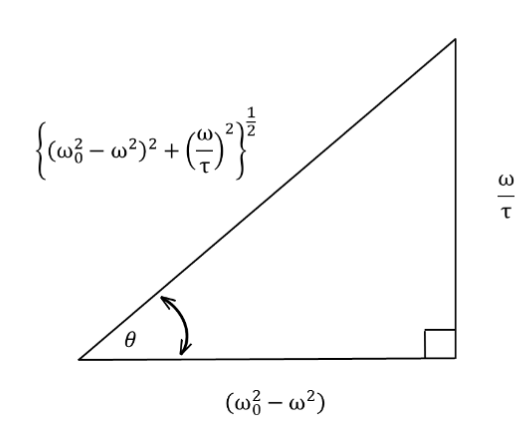
\includegraphics[scale=0.4]{pyth.png}
\end{figure}
\begin{align}
	\frac{\tx}{\tilde{\E}} &= \frac{qe^{i\theta}}{m\sqrt{(\om_0^2 - \om^2) + \left(\frac{\om}{\tau}\right)^2}} \\
	\tan\theta &= \frac{\om}{\tau(\om_0^2 - \om^2)} \\
	\cos\theta &= \frac{\om^2 - \om_0^2}{\sqrt{(\om^2 - \om_0^2)^2 + \left(\frac{\om}{\tau}\right)^2}} \\
	\sin\theta &= \frac{\om}{\tau\sqrt{(\om^2 - \om_0^2) + \left(\frac{\om}{\tau}\right)^2}}
\end{align}
Writing the definition of $\unl{P}$ (polarisation), and $\er$ (permittivity) in complex form:
\begin{equation}
	\tilde{\unl{P}} = (\er - 1)\eno\tilde{\uE} = Nq\tx
\end{equation}
Using $e^{i\theta} = \cos\theta + i\sin\theta$, the real and imaginary parts of the relative permittivity are:
\begin{align}
	\e_{real} &= 1 + \frac{Nq^2}{m\eno}\left(\frac{\om_0^2 - \om^2}{(\om_0^2 - \om^2)^2 + \left(\frac{\om}{\tau}\right)^2}\right) \\
	\e_{im} &= -\frac{Nq^2}{m\eno\tau}\frac{\om}{(\om_0^2 - \om^2) + \left(\frac{\om}{\tau}\right)^2}
\end{align}
\begin{figure}[H]
	\centering
	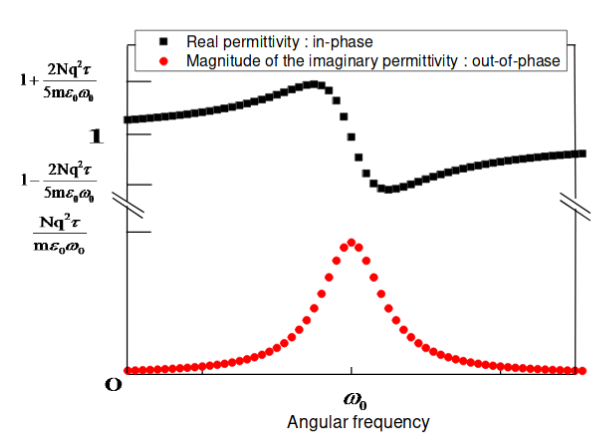
\includegraphics[scale=0.4]{angfreq.png}
\end{figure}

\chapter{}
\section{Auxiliary Fields and the Poynting vector}
\subsection{Electric Displacement Field}
\begin{equation}
	\unl{D} = \eno\uE + \unl{P}
\end{equation}
Rewriting this in differential form:
\begin{equation}
	\del\cdot\unl{D} = \del\cdot(\eno\uE+\unl{P}) = \rho_{total} - \rho_{dielectric} = \rho_{free}
\end{equation}
So we can rewrite Maxwell \RN{1} in terms of $\unl{D}$ and $\rho_{free}$:
\begin{equation}
	\del\cdot\unl{D} = \rho_{free}
\end{equation}
In general, we tend to use the relative permittivity to characterise a dielectric.
However, we can use $\unl{P}$ or $\unl{D} = \eno\uE + \unl{P} = \er\eno\uE$ if it simplifies calculations.

\subsection{Magnetic Field Strength}
\begin{equation}
	\uB = \mu_0(\unl{H}+\unl{M})
\end{equation}
Maxwell \RN{4} is
\begin{equation}
	\del\times\uB = \mu_0\J + \mu_0\eno\frac{\p \uE}{\p t}
\end{equation}
The current density produced by conducting, magnetic, and dielectric materials is given by
\begin{equation}
	\J = \J_{free} + \frac{\p\unl{P}}{\p t} + \del\times\unl{M}
\end{equation}
which can be rearranged as
\begin{equation}
	\del\times(\uB-\mu_0\unl{M}) = \mu_0\J_{free} + \mu_0\frac{\p}{\p t}(\unl{P} + \eno\uE)
\end{equation}
So we can rewrite Maxwell \RN{4} as:
\begin{equation}
	\del\times\unl{H} = \J_{free} + \frac{\p\unl{D}}{\p t}
\end{equation}
Again, we tend to use $\mu_r$ to characterise a magnetic material, however we can use $\unl{H}$ or $\unl{M}$ if it simplifies calculations.
\begin{align}
	\del\cdot\unl{D} &= \rho_{free} \tag{M\RN{1}} \\
	\del\cdot\uB &= 0 \tag{M\RN{2}} \\
	\del\times\uE &= -\frac{\p\uB}{\p t} \tag{M\RN{3}} \\
	\del\times\unl{H} &= \J_{free} + \frac{\p\unl{D}}{\p t} \tag{M\RN{4}}
\end{align}
\section{The Poynting Vector}
The direction of propagation for an electromagnetic waves is $\uE\times\unl{H}$.
Poynting suggested that the instantaneous power per unit area for electromagnetic waves is given by $\unl{N}$ where:
\begin{equation}
	\unl{N} = \uE\times\unl{H}
\end{equation}
\subsection{General Proof}
If $\unl{N}$ is the instantaneous power per unit area associated with electromagnetic fields, then the total energy per unit time radiating out of an arbitrary volume ($P_{rad}$) is
\begin{equation}
	P_{rad} = \int \unl{N}\cdot d\unl{S} = \int (\uE\times\unl{H})\cdot d\unl{S}
\end{equation}
Using the divergence theorem:
\begin{equation}
	P_{rad} = \int \del\cdot\unl{N}\,dV = \int \del\cdot(\uE\times\unl{H})\,dV
\end{equation}
Use the vector identity
\begin{equation}
	\del\cdot(\uE\times\unl{H}) = \unl{H}\cdot(\del\times\uE) - \uE\cdot(\del\times\unl{H})
\end{equation}
Hence, we have
\begin{equation}
	P_{rad} = \int \unl{H}\cdot(\del\times\uE)\,dV - \int \uE\cdot(\del\times\unl{H})\,dV
\end{equation}
From Maxwell's equations
\begin{align}
	\del\times\uE &= -\frac{\p\uB}{\p t} = -\mu_0\mu_r\frac{\p\unl{H}}{\p t} \\
	\del\times\unl{H} &= \J_{free} + \frac{\p \unl{D}}{\p t} = \J_{free} + \er\eno\frac{\p\uE}{\p t} \\
	P_{rad} &= \int \unl{H}\cdot\mu_r\mu_0\frac{\p\unl{H}}{\p t}\,dV - \int \uE\cdot\left(\J_{free} + \eno\er\frac{\p\uE}{\p t}\right)\,dV \\
	&= -\frac{\p}{\p t}\int \left(\frac{1}{2}\mu_r\mu_0H^2(t) + \frac{1}{2}\eno\er E^2(t)\right)\,dV - \int \uE\cdot\J\,dV \\
	\implies P_{rad} + \int \underbrace{\uE\cdot\J\,dV}_{\text{\shortstack{Power dissipated \\ as Joule heat}}} &= -\frac{\p}{\p t}\int \underbrace{\left(\frac{1}{2}\mu_r\mu_0H^2(t) + \frac{1}{2}\eno\er E^2(t)\right)\,dV}_{\text{\shortstack{Energy stored per unit volume in \\ the magnetic and electric fields}}}
\end{align}
The interpretation of the equation for $P_{rad}$ is:
\begin{itemize}
	\item The reduction in the potential energy stored in the electric and magnetic fields per unit time is equal to the net flow of power out through the surface plus the power dissipated as heat within the volume.
	\item The deviation is a self-consistent statement of the conservation of energy, so $\unl{N}$ correctly represents the instantaneous power per unit area.
\end{itemize}

\chapter{}
\section{Radiation and Communication}
\subsection{Maxwell's equations rewritten using potentials}
For time-independent problems, we use
\begin{equation}
	\uE = -\del V
\end{equation}
where $V$ is the electrostatic potential. \\
In general, the potential, $V$, is defined by:
\begin{equation}
	\uE = -\del V - \frac{\p \A}{\p t}
\end{equation}
Similarly, the magnetic vector potential is defined by:
\begin{equation}
	\uB = \del\times\A
\end{equation}
Consider Maxwell \RN{2}:
\begin{equation}
	\del\cdot\uB = 0 \because \del\cdot(\del\times\A) = 0
\end{equation}
Now consider Maxwell \RN{3}:
\begin{equation}
	\del\times\uE = \del\times\left(-\del V - \frac{\p\A}{\p t}\right) = -\del\times\del V - \frac{\p}{\p t}\del\times\A = -\frac{\p \uB}{\p t}
\end{equation}
Hence, if we rewrite $\uB$ and $\uE$ in terms of $\A$ and $V$, Maxwell \RN{2} and \RN{3} are automatically solved.
Maxwell's four equations are thus reduced to just two equations:
\begin{align}
	-\del\cdot\del V &- \frac{\p}{\p t}\del\cdot\A = \frac{\rho}{\eno}  \tag{M\RN{1}} \\
	\del\times\del\times\A &= \mu_0\J + \mu_0\eno\frac{\p}{\p t}\left(-\del V - \frac{\p\A}{\p t}\right) \tag{M\RN{4}}
\end{align}
The potentials $\A$ and $V$ are not uniquely specified.
We can add to the vector field $\A$ any function whose curl is zero, and add to $V$ any function whose gradient is zero.
Hence it is often useful to impose the Lorentz condition,
\begin{equation}
	\del\cdot\A = -\mu_0\eno\frac{\p V}{\p t}
\end{equation}
Maxwell \RN{1} becomes the wave equation for $V$:
\begin{equation}
	-\nabla^2V + \mu_0\eno\frac{\p^2V}{\p t^2} = \frac{\rho}{\eno}
\end{equation}
and Maxwell \RN{4} becomes the wave equation for $\A$:
\begin{equation}
	-\nabla^2\A + \mu_0\eno\frac{\p^2\A}{\p t} = \mu_0\J
\end{equation}

\subsection{Hertzian dipoles/oscillating electric dipoles}
A Hertzian dipole:
\begin{itemize}
	\item A length of wire in which a time-dependent alternating current is flowing (equivalent to an alternating electric dipole)
\end{itemize}
We can start to solve the wave equation for $\A$ by considering (static) solutions for
\begin{equation}
	-\nabla^2\A = \mu_0\J
\end{equation}
From electrostatics, using $\uE = -\nabla V$, we know the solution for $\del\cdot\uE = -\nabla\cdot\nabla V = -\nabla^2V = \frac{\rho}{\eno}$ is $V = \frac{Q}{4\pi\eno r}$, where $Q = \int \rho\,dV$. \\
By inspection, the static solution for $\A$ is:
\begin{equation}
	\A = \frac{\mu_0 I\,d\unl{l}}{4\pi},~ I\,d\unl{l} = \int \J\cdot dV
\end{equation}
Recognising that if we set $\J$ to be zero, we find oscillating solutions.
The general solution to the wave equation for $\A$ is:
\begin{equation}
	\A = \frac{\mu_0I\,d\unl{l}}{4\pi}e^{i(kr - \om t)}
\end{equation}
In spherical polar coordinates, $d\unl{l} = \cos\theta\hr - \sin\theta\hat{\theta}$.
Using $\uB - \del\times\A$, we have:
\begin{equation}
	\uB = \frac{\mu_0I}{4\pi}(1 - ikr)\sin\theta e^{i(kr - \om t)}\hat{\phi}
\end{equation}
We find physical solutions by taking the real parts of $\uB$.
There is a 'near-field' term that dominates close to the dipole and a 'far-field' term that describes the radiation distant from the dipole:
\begin{align}
	\uB_{near} &= \frac{\mu_0I}{4\pi r^2}\sin\theta \cos(kr - \om t)\hat{\phi} \\
	\uB_{far} &= \frac{\mu_0I}{4\pi r}k\sin\theta\sin(kr - \om t)\hat{\phi}
\end{align}
\begin{itemize}
	\item The near-field part originates from the quasi-static field produced by the moving charges.
	\item The far-field comes from changing current, associated with the acceleration of the charges, and cause the radiation.
\end{itemize}
Writing down Maxwell \RN{4} for the regions where there is no charge or current, we have $\del\times\uB = \mu_0\J + \mu_0\eno\frac{\p\uE}{\p t}$ which leads to:
\begin{align}
	\uE &= \frac{i}{\mu_0\eno\om}\del\times\uB \\
	&= \frac{\mu_0I}{2\pi}\frac{(i + kr)\cos\theta}{k^2r^3}e^{i(kr - \om t)}\hr + \frac{\mu_0I}{4\pi}\frac{(i+kriik^2r^2)\sin\theta}{k^2r^3}e^{i(kr - \om t)}\hat{\theta} \\
	\uE_{near} &= -\frac{\mu_0I}{2\pi r^2}\frac{\om}{k^2}\cos\theta\sin(kr - \om t)\hr - \frac{\mu_0I}{4\pi r^3}\frac{v}{k^2}\sin\theta\sin(kr - \om t)\hat{\theta} \\
	\uE_{far} &= -\frac{\mu_0I}{4\pi r}\om\sin\theta\sin(kr - \om t)\hat{\theta}
\end{align}

\chapter{}
Some notes:
\begin{itemize}
	\item $\uB_{near}$ and $\uE_{near}$ are $\frac{\pi}{2}$ out of phase with each other because the current reaches a maximum as the charges cross each other at maximum velocity.
	\item The electric field reaches a maximum when the electric dipole is at a maximum and the charges have a maximum separation.
	\item In contrast, $\uB_{far}$ and $\uE_{far}$ are in phase with each other - distant from the Hertzian dipole, we have plane waves. $\uE$ is vertically polarised when $\theta = \frac{\pi}{2}$, and $\uB$ is horizontally polarised.
\end{itemize}

\section{Production of a wave}
\begin{figure}[H]
	\centering
	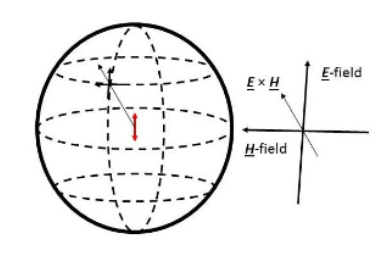
\includegraphics[scale=0.4]{bhmfield.png}
	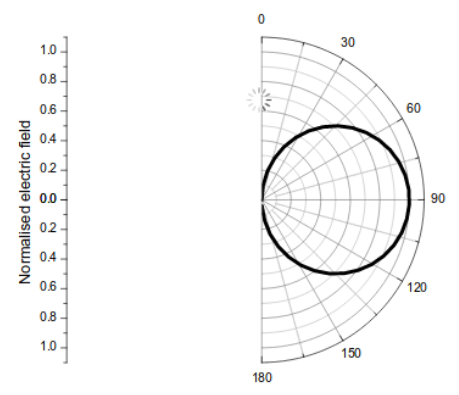
\includegraphics[scale=0.4]{normtheta.png}
\end{figure}
\begin{figure}[H]
	\centering
	\begin{subfigure}[b]{0.2\textwidth}
		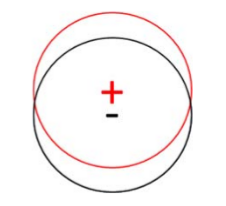
\includegraphics[scale=0.3]{waveprod1.png}
		\caption{}
	\end{subfigure}
	\begin{subfigure}[b]{0.35\textwidth}
		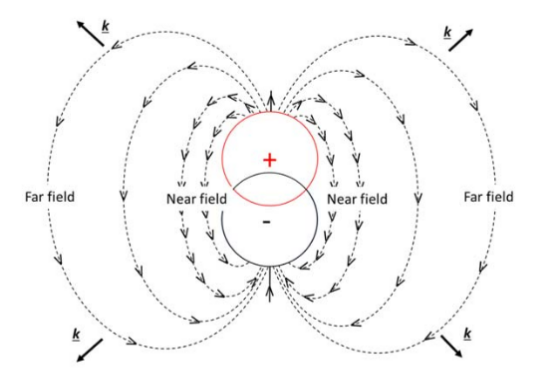
\includegraphics[scale=0.3]{waveprod2.png}
		\caption{}
	\end{subfigure}
	\begin{subfigure}[b]{0.35\textwidth}
		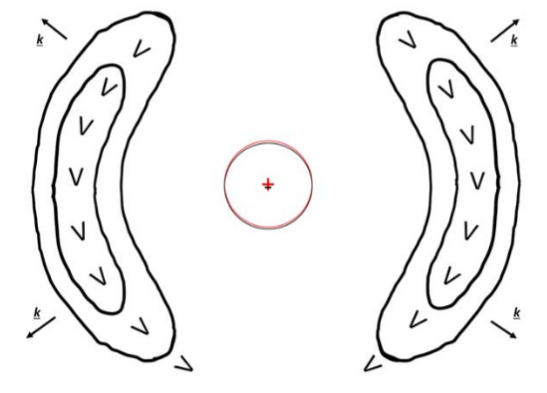
\includegraphics[scale=0.3]{waveprod3.png}
		\caption{}
	\end{subfigure}
\end{figure}

The production of the first half of a wave in snapshots:
\begin{enumerate}
	\item The charges separate and there are $\uE$-fields close to the charges.
	\item V-shaped chevrons and the dotted lines show the electric field lines.
	For any snapshot in time, the charges behave like an extended dipole with both near- and far-field terms contributing to the $\uE$-field.
	\item The first half wave separates and radiates from the dipole.
	The solid lines are contours.
	The $\uE$-field points in the positive $\theta$ direction through the first half wave.
\end{enumerate}

\begin{figure}[H]
	\centering
	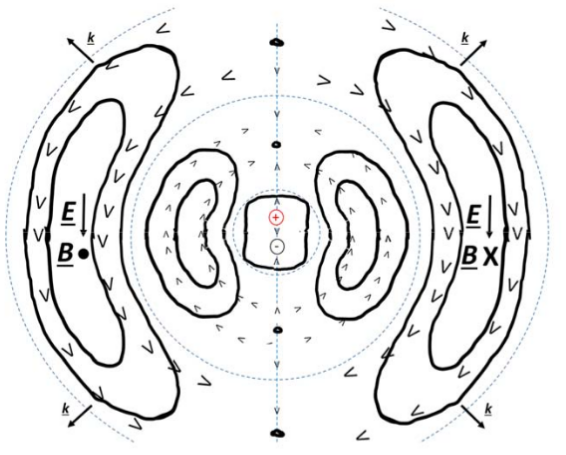
\includegraphics[scale=0.4]{waveprod.png}
\end{figure}

\begin{itemize}
	\item The solid lines are contours.
	\item Each magnetic field line is a circle with a dipole along the axis.
	\item The cross product $\uE\times\uB$ gives the direction of propagation.
\end{itemize}

\section{The angular dependence of the power radiated by a Hertzian dipole}
We know that the instantaneous power radiated per unit area in any direction is
\begin{equation}
	\unl{N} = \uE\times\unl{H}
\end{equation}
The angular dependence of the time-averaged power unit area is:
\begin{equation}
	\unl{N}_{t-av} = |\uE\times\unl{H}|_{t-av} = \frac{1}{2}\frac{\mu_0cI_0^2(\delta l)^2\sin^2\theta}{4r^2\lam^2}\hr
\end{equation}
This is from the far-field limit for $\uB_{far}$ and $\uE_{far}$. \\
$\sin^2 > 0$ so the time average is $\frac{1}{2}$ from $1 = \cos^2x + \sin^2x$ when time-averaged.

The power peaks in the equatorial plane ($\theta = \frac{\pi}{2}$).
No power is radiated along the axis of the dipole ($\theta = 0,\pi$).

\chapter{}
\section{The total time-averaged power radiated by a Hertzian dipole}
\begin{align}
	P_{total} &= \frac{1}{2}\int\int \frac{1}{2}\frac{\mu_0cI_0^2(\delta l)^2\sin^2\theta}{4r^2\lam^2}r^2\sin\theta\,d\theta\,d\phi \\
	          &= \frac{\mu_0cI_0^2(\delta l)^2}{8\lam^2}\int_0^\pi \sin^3\theta\,d\theta \int_0^{2\pi} d\phi \\
           	  &= \frac{\mu_0c\pi}{3}\left(\frac{\delta l}{\lam}\right)I_0^2
\end{align}

\section{Electromagnetic fields and wave crossing interfaces}
\textbf{Pauli}: \emph{"God made the bulk, but the devil has the surfaces."}

\subsection{Boundary conditions across the interfacial plane between two dielectrics}

\begin{figure}[H]
  	\centering
  	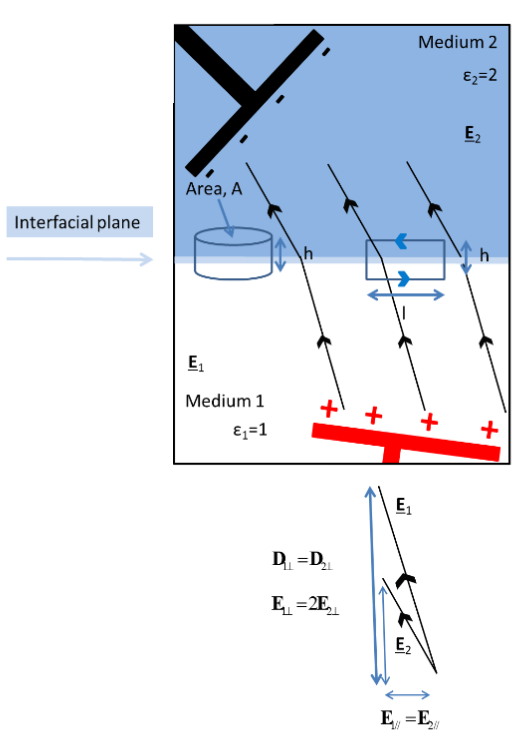
\includegraphics[scale=0.4]{wolfgang.png}
\end{figure}

Two charged capacitor plates immersed in two dielectrics.
The magnitude and direction of the dc electric field changes as it passes from one dielectric to another.
(N.b. This is not a ray dispersion.)

\begin{enumerate}
	\item From an insulating material, consider the cylinder and Maxwell \RN{1}:
	\begin{align}
		\del\cdot\unl{D} &= \rho_{free} = 0 \\
		\lim_{h\to0} \int \unl{D}_1\cdot d\unl{S} &= \int \unl{D}_2\cdot d\unl{S} \\
		\implies D_{1\perp} &= D_{2\perp} \\
		\implies \e_1\E_{1\perp} &= \e_2\E_{2\perp}
	\end{align}
	\item Using Maxwell \RN{3} (consider the path drawn):
	\begin{align}
		\del\times\uE &= -\frac{\p \uB}{\p t} \\
		\int \uE\cdot d\unl{l} &= -\frac{\p}{\p t}\int \uB\cdot d\unl{S} \\
		\lim_{h\to0} (\E_{1\parallel} \int - \E_{2\parallel}\int) &= -\frac{\p\phi}{\p t} = 0 \\
		\implies \E_{1\parallel} = \E_{2\parallel}
	\end{align}
\end{enumerate}


\chapter{}
\section{Boundary conditions across the interfacial plane between two magnetic materials}

\begin{figure}[H]
  	\centering
  	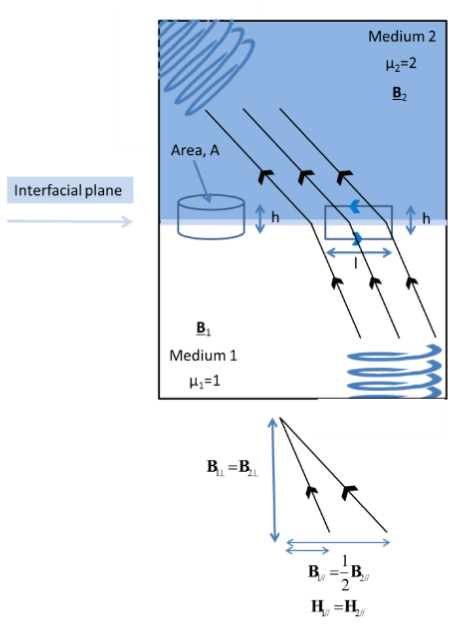
\includegraphics[scale=0.4]{wolfgang2.png}
\end{figure}

Maxwell \RN{2}:
\begin{equation}
	\int \uB\cdot d\unl{S} = 0 \implies \B_{1\perp} = \B_{2\perp}
\end{equation}
Maxwell \RN{4}:
\begin{align}
	\del\times\uB &= \mu_0\J + \mu_0\eno\frac{\p\uE}{\p t} \\
	\del\times\unl{H} = \J_{free} + \frac{\p\unl{D}}{\p t} \\
	\int \unl{H}\cdot d\unl{l} = \int \J_{free}\cdot d\unl{S} + \frac{p}{\p t}\int \del\cdot\unl{D}\,dV
\end{align}
RHS equal to zero:
\begin{itemize}
	\item no free current density
	\item no free charge density
\end{itemize}
\begin{equation}
	\implies H_{1\parallel} = H_{2\parallel}
\end{equation}

\section{The laws of geometrical optics}

\begin{figure}[H]
	\centering
	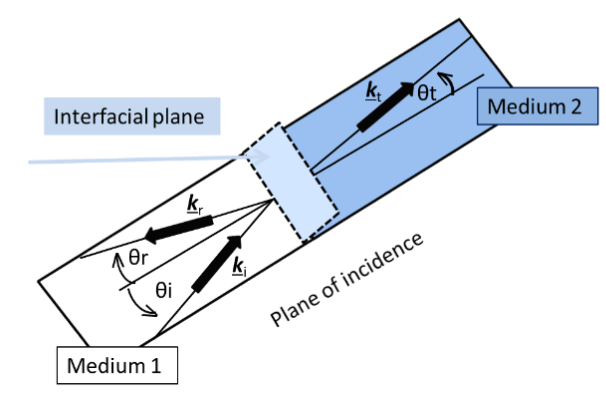
\includegraphics[scale=0.4]{geolaw.png}
\end{figure}

An electromagnetic wave incident on an interface - it is partially reflected and partially transmitted.
Let's make no assumptions about the polarisation of the reflected and transmitted wave:
\begin{align}
	\uE_i(\vr,t) &= \uE_{0i}\exp[i(\vec{k}_i\cdot\vr - \om_it)] \\
	\uE_r(\vr,t) &= \uE_{0r}\exp[i(\vec{k}_r\cdot\vr - \om_rt)] \\
	\uE_t(\vr,t) &= \uE_{0t}\exp[i(\vec{k}_t\cdot\vr - \om_tt)]
\end{align}
The $\uE_0$ and $\vec{k}$ terms are constants, not variables.
$\vec{k}$ can in principle be complex, to incorporate phase information and decay.

\begin{figure}[H]
	\centering
	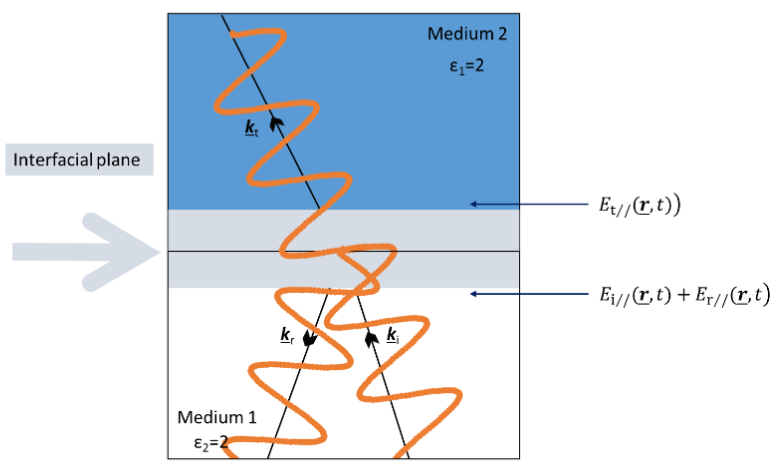
\includegraphics[scale=0.4]{geolaw2.png}
\end{figure}

Across the interfacial plane, the general condition for the continuity of $\E_{\parallel}$ (i.e. $\E$ parallel to the interfacial plane) requires:
\begin{equation}
	\E_{i\parallel} (\vr,t) + \E_{r\parallel} = \E_{t\parallel}(\vr,t)
\end{equation}
for all $\vr$ in the interfacial plane at all $t$.

For simplicity, we assume the origin of the coordinate system is in the interfacial plane and consider special cases:
\begin{enumerate}
	\item $r=0$:
	\begin{align}
		\E_{0i\parallel}e^{-i\om_it} &+ \E_{0r\parallel}e^{-i\om_rt} = \E_{0t\parallel}e^{-\om_tt} \\
		\E_{0i\parallel}\cos(\om_it) &+ \E_{0r\parallel}\cos(\om_rt) = \E_{0t\parallel}\cos(\om_tt)
	\end{align}
	where $\E_{0i\parallel},\E_{0r\parallel},\E_{0t\parallel}$ are all constants

	An argand diagram showing these arbitrary complex vectors where at $t=1$, $r_1e^{i\theta_1t} + r_2e^{i\theta_2t} = r_3e^{i\theta_3t}$.
	Also shown are the three complex vectors at a later time where the magnitude of the vectors has remained constant but the phase of each complex vector has doubled (i.e. $t=2$).
	\begin{itemize}
		\item LHS - At the later time the vector addition identity is still valid because $\theta_1 = \theta_2 = \theta+3$ and remains true at all times.
		\item RHS - At the later $t=2$, the vector addition identity is no longer true.
	\end{itemize}
	Hence, given the vector equality must be true at all times, the phases of each complex wave must be the same, so:
	\begin{equation}
		\om_i = \om_r = \om_t
	\end{equation}
	(i.e. the incident, transmitted, and reflected waves all have the same angular frequency)

	\begin{figure}[H]
		\centering
		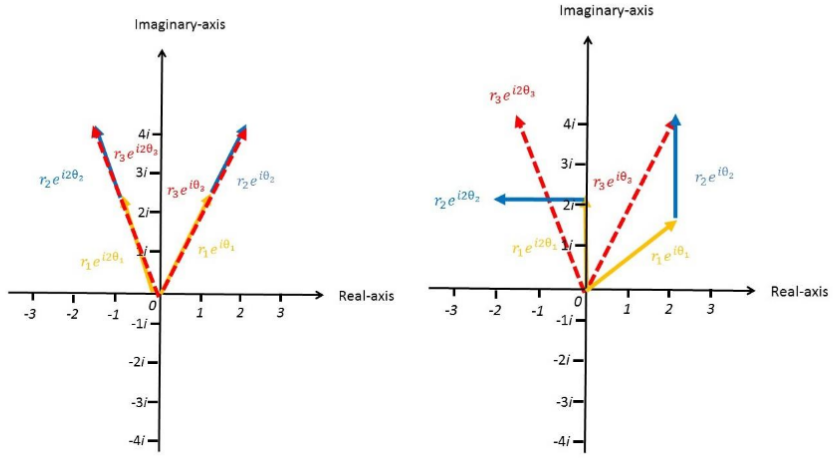
\includegraphics[scale=0.4]{argand.png}
	\end{figure}

	\item $t=0$:
	\begin{equation}
		\E_{0i\parallel}e^{i(\vk_i\cdot\vr)} + \E_{0r\parallel}e^{i(\vk_r\cdot\vr)} = \E_{0t\parallel}e^{i(\vk_t\cdot\vr)}
	\end{equation}
	The condition is true for all $\vr$ in the plane.
	\begin{equation}
		\implies \vk_i\cdot\vr = \vk_r\cdot\vr = \vk_t\cdot\vr
	\end{equation}
\end{enumerate}
Consider reflection (i.e. $(\vk_i - \vk_r)\cdot\vr = 0$) $\implies$ $\vk_i - \vk_r$ is normal to the interface. Then:
\begin{equation}
	\vk_{i\parallel} = \vk_{r\parallel}
\end{equation}
Since the phase velocities are the same for the incident and reflected waves:
\begin{align}
	|\vk_r| &= |\vk_r| \\
	\implies \theta_i = \theta_r
\end{align}
The first law of geometrical optics: the angle of reflection $=$ the angle of incidence.

Consider transmission (i.e. $\vk_r\cdot\vr = \vk_t\cdot\vr$):
\begin{align}
	(\vk_i &- \vk_t)\cdot\vr = 0 \\
	\vk_{i\parallel} &= \vk_{t\parallel} \\
	\vk_i\sin\theta_i &= \vk_t\sin\theta_t
\end{align}
Using the definition of the refractive index, $n_i = \frac{c}{v_{phase}} = \frac{c\vk_i}{\om}, n_t = \frac{c\vk_t}{\om}$:
\begin{equation}
	\frac{n_i}{n_t} = \frac{k_i}{k_t} = \frac{\sin\theta_t}{\sin\theta_i} \tag{Snell's Law}
\end{equation}
Snell's Law is the second law of geometrical optics.

\chapter{}
Snells Law is valid for all polarisations.
Since we can also write down
\begin{align}
	\vk_r\cdot \vr &= \vk_t\cdot \vr \\
	(\vk_r - \vk_t)\cdot\vr &= 0 \\
	\vk_r\sin\theta_r &= \vk_t\sin\theta_t
\end{align}
The constraints on the components of the incident, reflected, and transmitted wavevectors parallel to the interfacial plane and the constraints on the magnitude of the wavevectors in both media lead to the third law of geometrical optics:
\begin{quote}
\emph{"The incident, reflected, and transmitted waves are all in the plane of incidence."}
\end{quote}

\section{Fresnel's Equations}
\subsection{Perpendicular Equations}
$\uE$-field normal to the plane of incidence.

\begin{figure}[H]
	\centering
	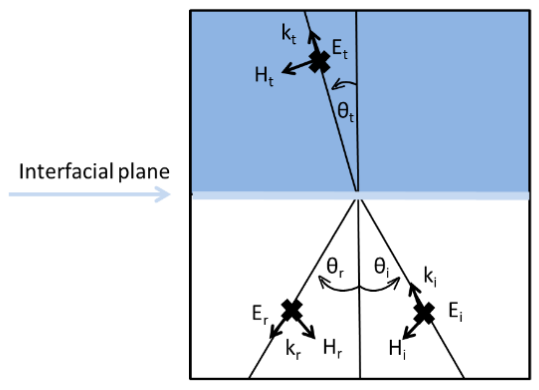
\includegraphics[scale=0.4]{normfres.png}
\end{figure}

Assume $\E$ doesn't change direction broadly in transmission and reflection - use $\uE \times \unl{H} \implies \vk$

An electromagnetic wave close to the interfacial plane incident to an interfacial plane where $\uE$ is normal to the plane of incidence.
The incident and reflective waves superimpose in medium 1, only the transmitted wave is in medium 2.


We use the convention that the direction of the $\uE$-field of the reflected and transmitted waves are broadly similar to the incident wave.
The continuity of $\uE$ parallel to the interfacial plane requires
\begin{equation}
	\E_{0i} + \E_{0r} = \E_{0t}
\end{equation}
The continuity of $\unl{H}$ parallel to the interfacial:
\begin{equation}
	H_{0i}\cos\theta_i - H_{0r}\cos\theta_r = H_{0t}\cos\theta_t
\end{equation}
We know that $\theta_i = \theta_r$ and $\om$ is constant.
Using $\del\times\uE = -\frac{\p\uB}{\p t} \implies \vk\times\uE = \om\uB$:
\begin{equation}
	\uB = \frac{\uE}{v_{phase}}
\end{equation}
The refractive index, $n$, by definition is:
\begin{equation}
	n = \frac{c}{v_{phase}} = \sqrt{\er\mu_r}
\end{equation}
Using $\uB = \mu_0\mu_r\unl{H} = \mu\unl{H}$
\begin{equation}
	\unl{H} = \frac{n\uE}{c\mu}
\end{equation}
Substituting Eq. 20.7 into Eq. 20.5, and assuming the media are non-magnetic (i.e. $\mu = \mu_0$):
\begin{equation}
	(n_i\E_{0i} - n_r\E_{0r})\cos\theta_i = n_t\E_{0t}\cos\theta_t
\end{equation}
Then combining Eq. 20.4 and Eq. 20.8 to eliminate $\E_{0t}$ and $\E_{0r}$ in turn, we obtain:
\begin{align}
	\frac{\E_{0r}}{\E_{0i}} &= \frac{n_i\cos\theta_i - n_t\cos\theta_t}{n_i\cos\theta_i + n_t\cos\theta_t} \\
	\frac{\E_{0t}}{\E_{0i}} &= \frac{2n_i\cos\theta_i}{n_i\cos\theta_i + n_t\cos\theta_t}
\end{align}
These are Fresnel's two equations for $\uE$ normal to the plane of incidence.

\subsection{Parallel Equations}

\begin{figure}[H]
	\centering
	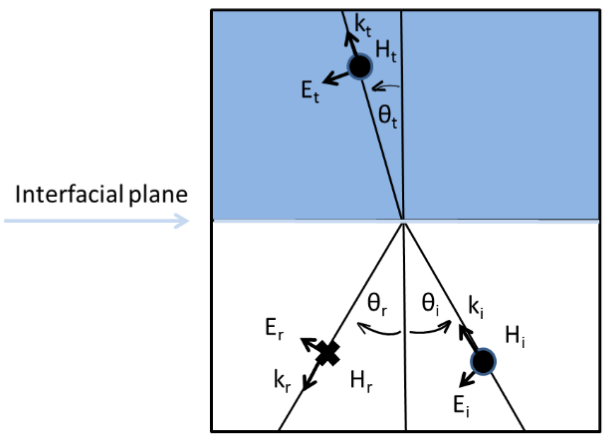
\includegraphics[scale=0.4]{parfres.png}
\end{figure}

The continuity equations for $H_{\parallel}$ and $\E_{\parallel}$ are now:
\begin{equation}
	(\E_{0i} + \E_{0r})\cos\theta_i = \E_{0t}\cos\theta_t
\end{equation}
$H$ is parallel to interfacial plane so,
\begin{align}
	H_{0i} - H_{0r} &= H_{0t} \\
	n_i(\E_{0i} + \E_{0r}) &= n_t\E_{0t}
\end{align}
So we find:
\begin{align}
	\frac{\E_{0r}}{\E_{0i}} &= \frac{n_i\cos\theta_t - n_t\cos\theta_i}{n_i\cos\theta_t + n_t\cos\theta_i} \\
	\frac{\E_{0t}}{\E_{0i}} &= \frac{2n_i\cos\theta_i}{n_i\cos\theta_t + n_t\cos\theta_t}
\end{align}
These are Fresnel's equations for $\uE$ parallel to the plane of incidence.

\begin{figure}[H]
	\centering
	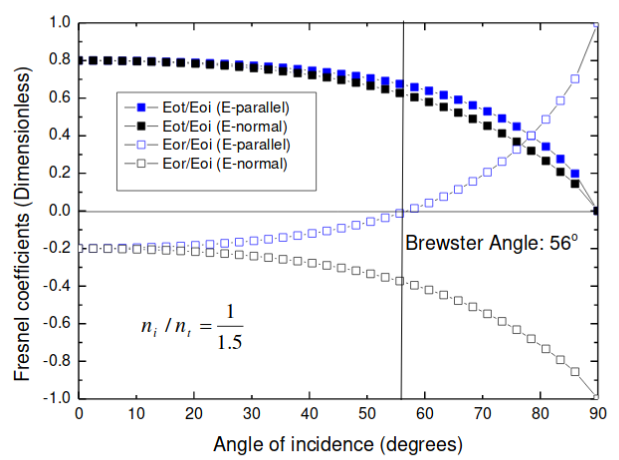
\includegraphics[scale=0.35]{brews.png}
	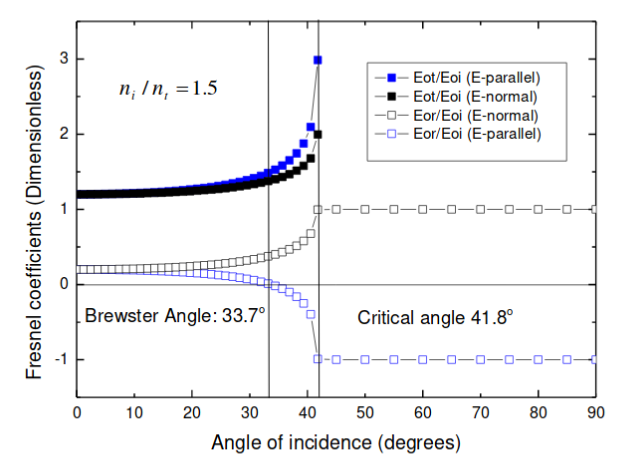
\includegraphics[scale=0.35]{crits.png} \\
	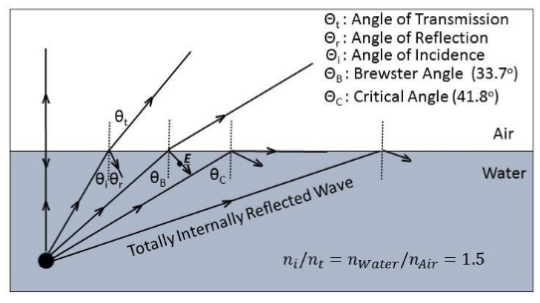
\includegraphics[scale=0.4]{tint.png}
\end{figure}

\section{Coefficient of reflection and transmission}
We can also consider reflection and transmission coefficients that are consistent with conservation of energy using the Poynting vector, $\unl{N} = \uE \times \unl{H}$ (instantaneous power per unit area).

For dielectrics (non-magnetic, non-conducting):
\begin{equation}
	\uB = \frac{\uE}{v_{phase}} \implies v_{phase} = \sqrt{\frac{1}{\er\eno\mu_0}}
\end{equation}
The average power per unit time per unit area incident on the interface (perpendicular to the direction of travel), $N_i$:
\begin{equation}
	N_i = \frac{1}{2}\left(\frac{\er}{\mu_0}\right)^{\frac{1}{2}} \E_{0i}^2\cos\theta_i
\end{equation}

\chapter{}
\section{Coefficients of reflection and transmission}
Incident:
\begin{align}
	\unl{N} &= \uE \times \unl{H} \\
	N_i &= \frac{1}{2}\left(\frac{\er}{\mu_0}\right)^{\frac{1}{2}} \E_{0r}^2\cos\theta_i
\end{align}
This is for the reflected wave, where $\cos\theta$ is using the angle between $\vk$ and $\hn$ to the interfacial plane:
\begin{equation}
	N_r = \frac{1}{2}\left(\frac{\e_1}{\mu_0}\right)^{\frac{1}{2}} \E_{0r}^2\cos\theta_r
\end{equation}
For the transmitted wave:
\begin{align}
	N_t &= \frac{1}{2}\left(\frac{\e_2}{\mu_0}\right)^{\frac{1}{2}} \E_{0t}^2\cos\theta_t \\
	R &= \frac{N_r}{N_i} = \left(\frac{\E_{0r}}{\E_{0i}}\right)^2
\end{align}
and the transmission coefficient is defined as:
\begin{equation}
	T = \frac{N_t}{N_i} = \left(\frac{\e_2}{\e_1}\right)^{\frac{1}{2}}\frac{\E_{0t}^2}{\E_{0i}^2} \frac{\cos\theta_t}{\cos\theta_i} = \frac{n_2}{n_1}\frac{\E_{0t}^2}{\E_{0i}^2} \frac{\cos\theta_t}{\cos\theta_i}
\end{equation}
Using Fresnel's equations in either polarisation gives:
\begin{equation}
	R + T = 1
\end{equation}

\section{Wave guides}
\subsection{Waves propagating in a hollow rectangular waveguide}

\begin{figure}[H]
	\centering
	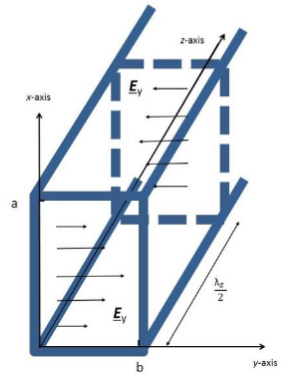
\includegraphics[scale=0.4]{box.png}
\end{figure}

A hollow waveguide carrying a transverse electric wave.
Transverse electromagnetic waves cannot exist inside a hollow waveguide.

Maxwell's equations give:
\begin{equation}
	\nabla^2\uE = \mu_0\eno\frac{\p^2\uE}{\p t^2}
\end{equation}
for propagation in the z-direction, we can first consider transverse $\E$-field (i.e. the $\E$-field perpendicular of propagation) and for simplicity take the $\E$-field to be in the y-direction only.
\begin{equation}
	\uE(\vr,t) = \hat{j}E_{0y}\exp[i(kz - \om t)]\sin(k_xx)
\end{equation}
The solution meets the requirement that the component on $\E$ parallel to the internal boundaries of the waveguide must be zero, else it generate currents which decays the $\E$-field so we need $\E = 0$ at boundaries for steady state.

For steady state solutions, the constraint on the component of $\E$-field parallel to the internal surface being zero requires
\begin{equation}
	k_xa = m\pi,~ m \in \mathcal{Z}
\end{equation}
The solution must satisfy the wave equation:
\begin{align}
	k^2 &+ k_x^2 = \frac{\om^2}{c^2} \\
	\implies k^2 &= \frac{\om^2}{c^2} - \frac{m^2\pi^2}{a^2}
\end{align}
This is the dispersion relation for EM waves in a waveguide. \\
$k^2 > 0$ for steady state, if $k$ is complex, leads to decay. \\
Similar to a plasma, we have a cut off for angular frequency (where $k = 0$) given by
\begin{equation}
	\om_c = \frac{\pi c}{a}
\end{equation}
We can identify two regions:
\begin{enumerate}
	\item $\om > \om_c$ - $k$ is real, wave can propagate without attenuation
	\item $\om < \om_c$ - $k$ is imaginary, there is an attenuated solution
\end{enumerate}

\subsection{Phase velocity}
\begin{align}
	v_{phase} &= \frac{\om}{k} = \frac{c}{\sqrt{1 - \left(\frac{\om_c}{\om}\right)^2}} > c, \text{ for } \om > \om_c \\
	v_{group} &= \frac{\p \om}{\p k} = c\sqrt{1 - \left(\frac{\om_c}{\om}\right)^2} < c \text{ for } \om > \om_c
\end{align}

\begin{figure}[H]
	\centering
	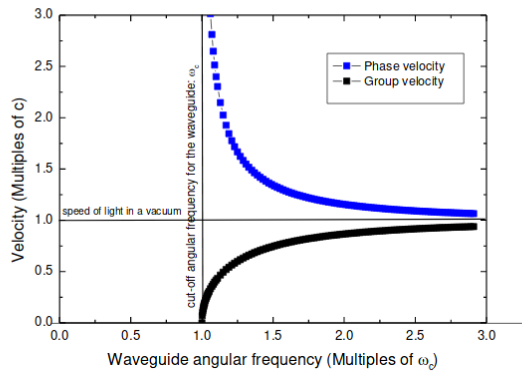
\includegraphics[scale=0.5]{phasegroup2.png}
\end{figure}

For the propagating wave, Maxwell \RN{3}:
\begin{align}
	\del \times \uE &= -\frac{\p\uB}{\p t} \\
	\del \times \uE &=
	\begin{vmatrix}
		\hat{i} & \hat{j} & \hat{k} \\
		\frac{\p}{\p x} & \frac{\p}{\p y} & \frac{\p}{\p z} \\
		\cancel{\E_x}^{\to 0} & \E_y & \cancel{\E_z}^{\to 0}
	\end{vmatrix}
	= -\hat{i}\frac{\p\E_y}{\p z} + \hat{k} \frac{\p E_y}{\p x} \\
	&= -ik\E_{0y}\exp[i(kz - \om t)]\sin(k_xx)\hat{i} + k_x\E_{0y}\exp[i(kz - \om t)]\cos(k_xx)\hat{k}
\end{align}
Maxwell \RN{3} gives
\begin{align}
	\uB &= \frac{1}{i\om}\del\times\uE \\
	\uB &= -\frac{\E_{0y}}{c}\sqrt{1 - \left(\frac{\om_c}{\om}\right)^2}\exp[i(kz - \om t)]\sin(k_xx)\hat{i} - \frac{i\om_c}{c\om}\E_{0y}\exp[i(kz - \om t)]\cos(k_xx)\hat{k}
\end{align}
$\B$-field has components parallel and perpendicular to $k$.

The first component is a transverse one, the second is longitudinal.

A transverse electric wave (TE) has an $\E$-field that is only transverse, but it has a $\B$-field that has components that are both transverse and parallel (longitudinal) to the direction of propagation.

A transverse magnetic wave has a $\B$-field that is transverse to the direction of propagation but an $\E$-field that has both transverse and longitudinal components.


















\end{document}
